%%%Presnetation for Aarhus, 11 October 2017

\documentclass[12pt, notes=show]{beamer}

\usetheme[width=0cm]{Goettingen}
\usecolortheme{rose}
\useoutertheme{default}
\setbeamerfont{caption}{size=\scriptsize}
\setbeamertemplate{navigation symbols}{}

%%change default colors
\definecolor{UPF}{RGB}{200,16,46}
\setbeamercolor{title}{fg=UPF}
\setbeamercolor{frametitle}{fg=UPF}
\setbeamercolor{structure}{fg=UPF}

%%To remove upper and lower beamer pane and add number of page
\addtobeamertemplate{navigation symbols}{}{%
	\usebeamerfont{footline}%
	\usebeamercolor[fg]{footline}%
	\hspace{1em}%
	$\dfrac{\insertframenumber}{\inserttotalframenumber}$
}

\usepackage{hyperref}
\usepackage{fontspec} 
\setsansfont{Futura LT}

\usepackage{array}

\usepackage{arydshln}
\usepackage{amsmath}

\usepackage{mathptmx}
\usepackage{latexsym}
\usepackage{mathtools}
\usepackage{multirow}
\usepackage{caption}
\usepackage{listings}

\usepackage[beamer,customcolors]{hf-tikz}
\usepackage{tabularx}
\usepackage{colortbl}

%%Tikz command used to annotate table
%
\newcounter{nodecount}

\newcolumntype{g}{>{\columncolor{red}}c}

\newcommand\tabnode[1]{%
    \addtocounter{nodecount}{1}%
    \tikz[remember picture,overlay]\node[inner sep=0pt] (\thenodecount) {#1};}
%
%%%%%%%%%%



\title{
	An agent-based model of trade in the Roman East (25BC-150AD) \\
	{\small Impact of social interactions on economic trends}
}

\institute{UrbNet seminar series\\ Aarhus, Octobre 2017}

\author{Simon Carrignon, Tom Brughmans \& Iza Romanowska}

\date{
	\scriptsize
	\begin{columns}
		\begin{column}{.3\textwidth}
			\begin{center}
				
\includegraphics[height=1cm]{../../logos/bscLogo.jpg} \hspace{2cm}
			\end{center}
		\end{column}
		\begin{column}{.3\textwidth}
			\begin{center}
				
\includegraphics[height=1cm]{../../logos/upf_word_imp.jpg} %declare logo image with an alias here 
			\end{center}
		\end{column}
	\end{columns}

}
\begin{document}
\begin{frame}
	\maketitle

\end{frame}

\section{Introduction}

\begin{frame}{ICRATES}
    \footnotesize
    \vspace{.5cm}
Change in distribution of Tableware in the  Roman East, 25BC 150AD:
\begin{columns}
    \begin{column}{.5\textwidth}
	\begin{itemize}
	    \item 5 types of wares 
	    \item Distribution among 222 sites
	    \item 5121 ware dataset
	\end{itemize}
    \end{column}
    \begin{column}{.5\textwidth}
	\centering
	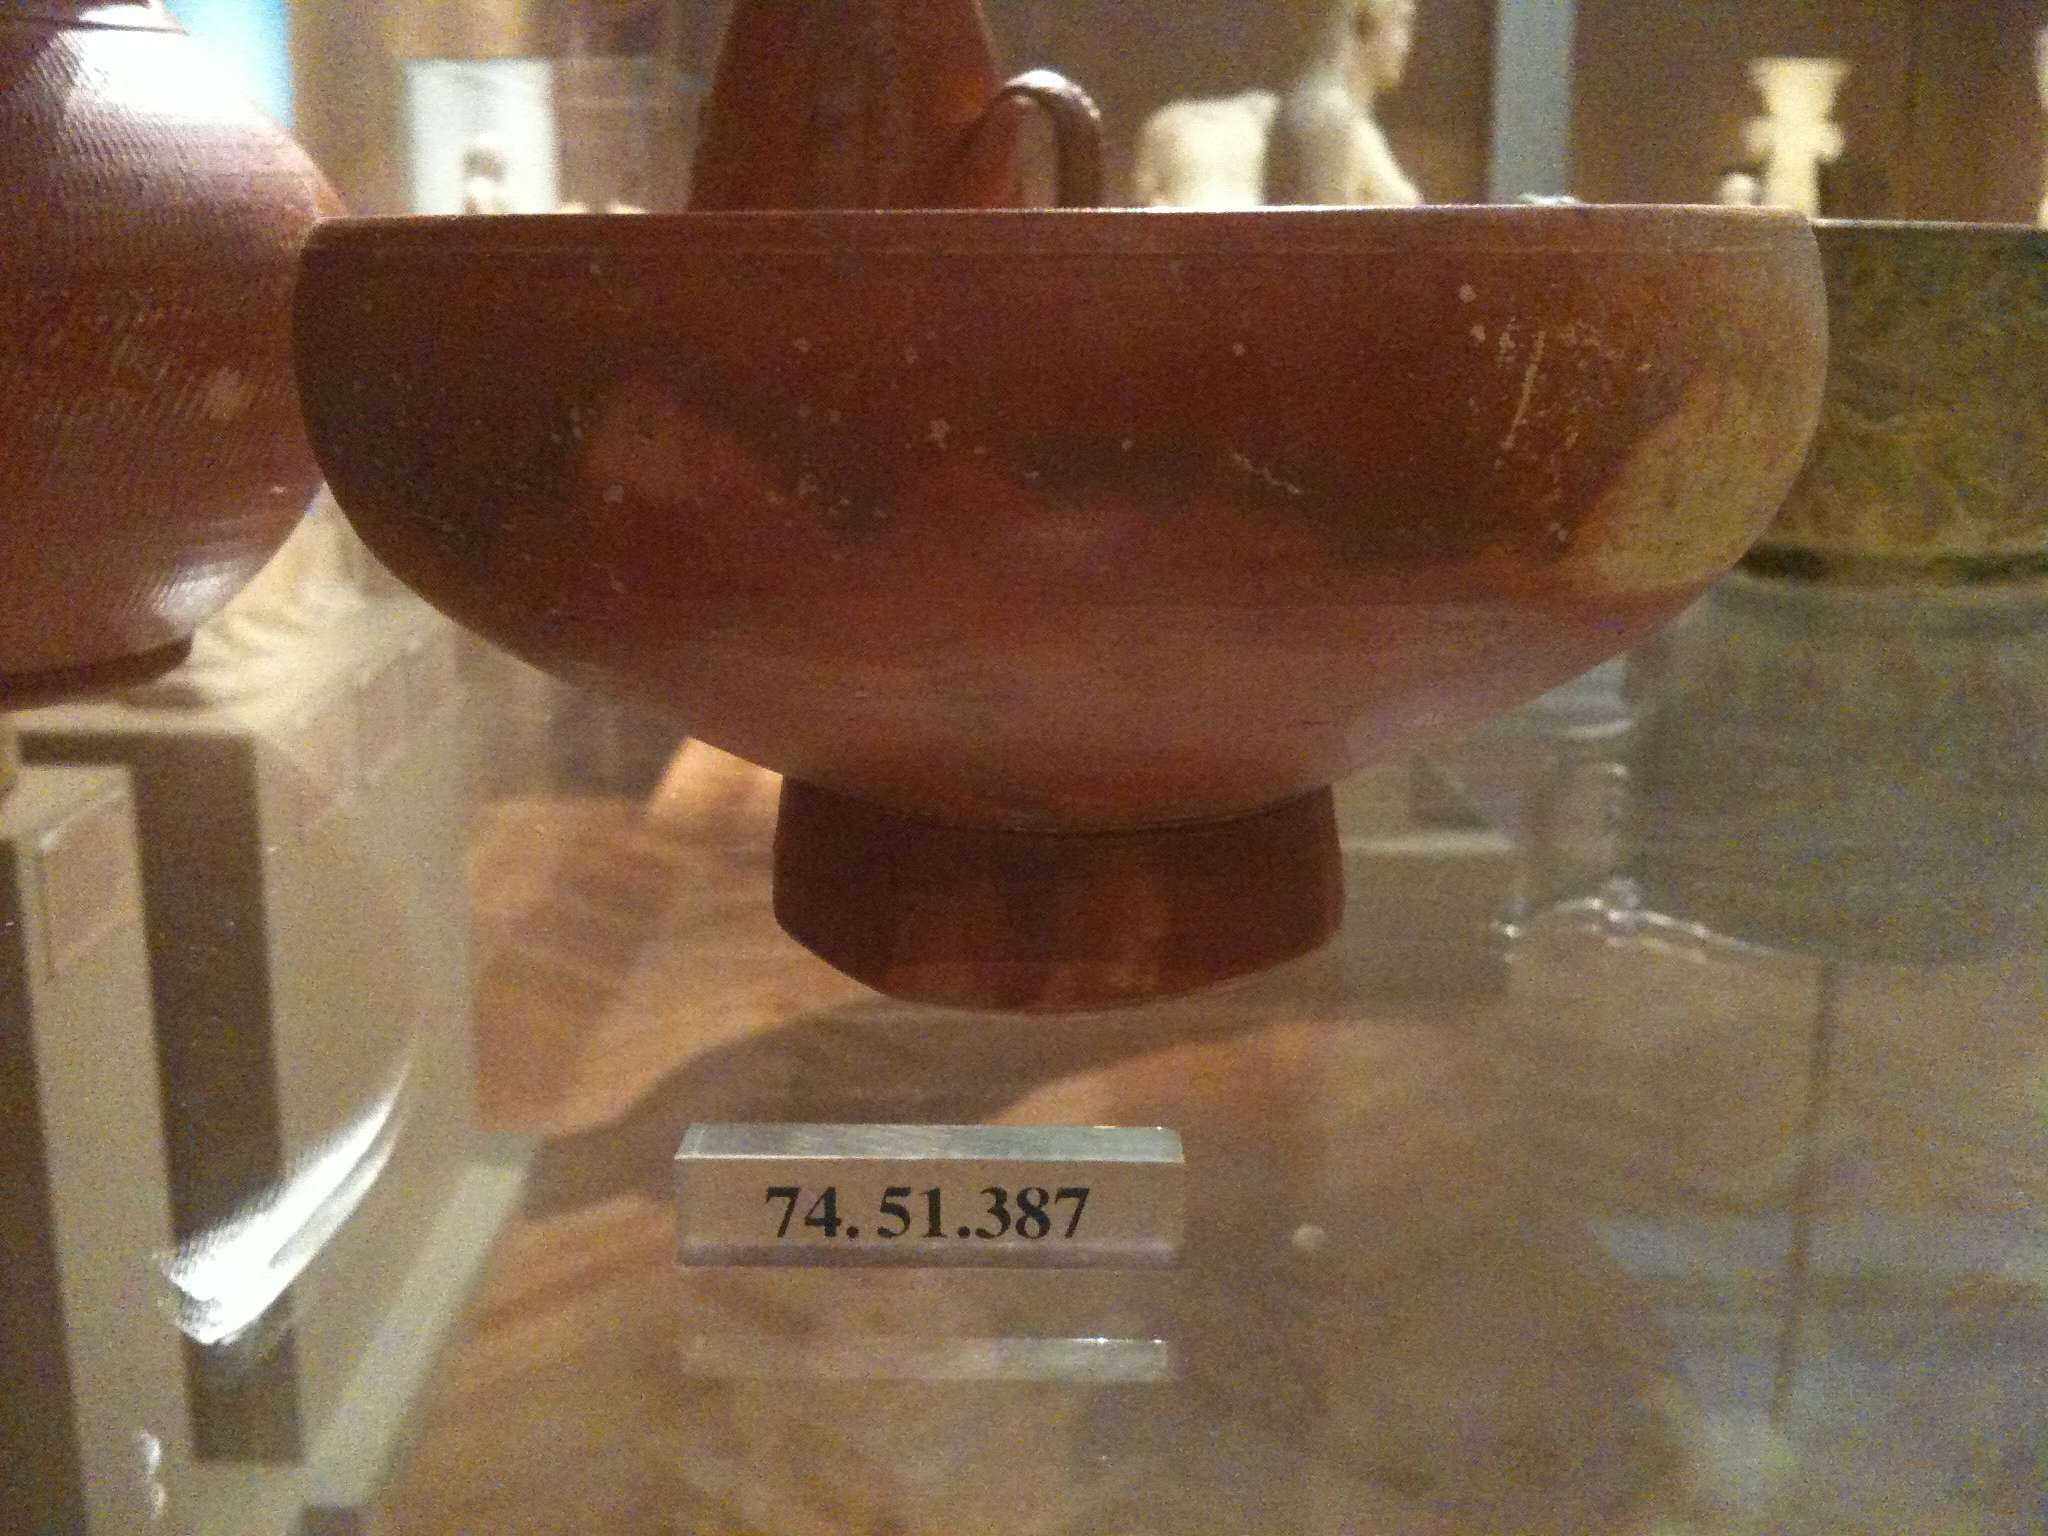
\includegraphics[width=.4\textwidth]{images/ESA_Metmuseum.jpg}\\
	\textit{\tiny Eastern sigillata A}
	
    \end{column}
\end{columns}

 \begin{figure}
     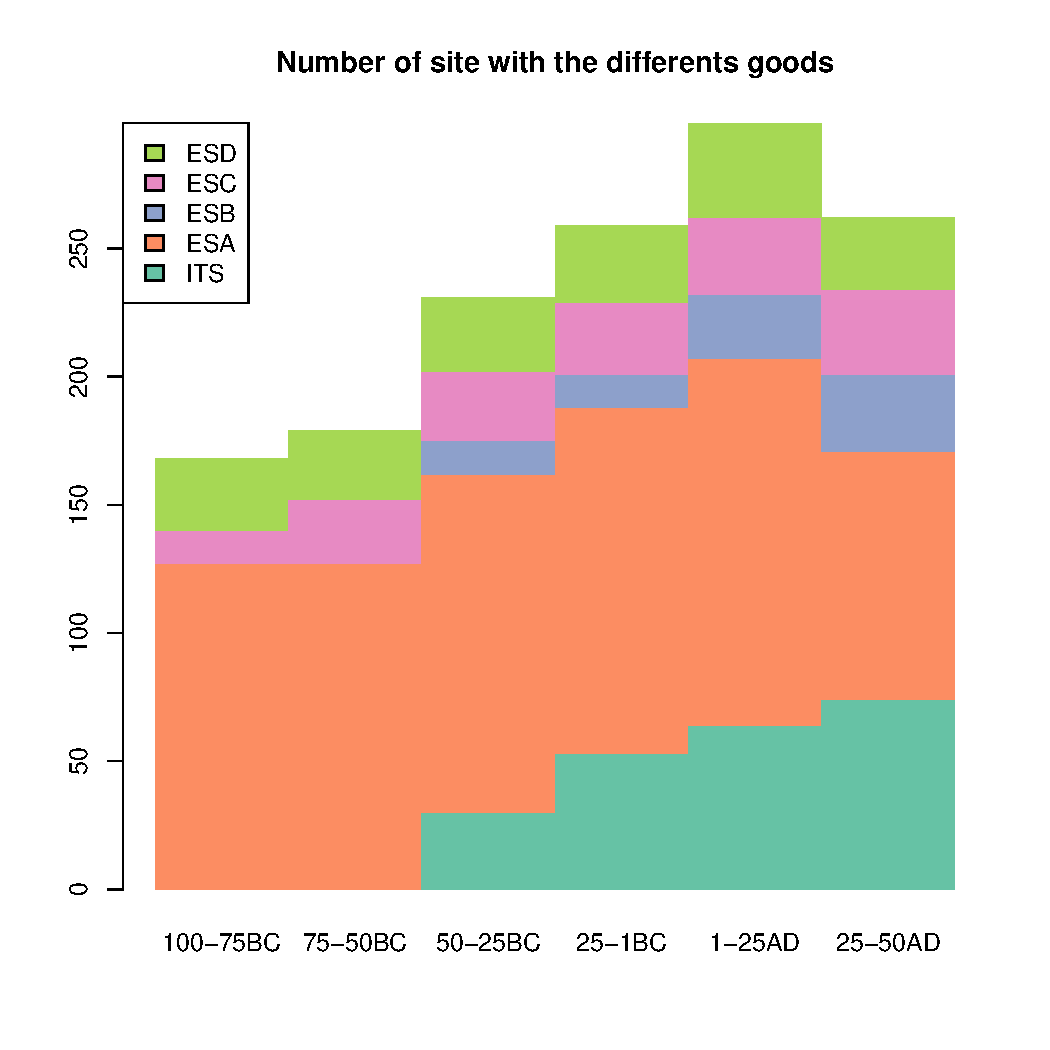
\includegraphics[width=.45\textwidth]{../images/hmNbSiteWGoodData.pdf}
     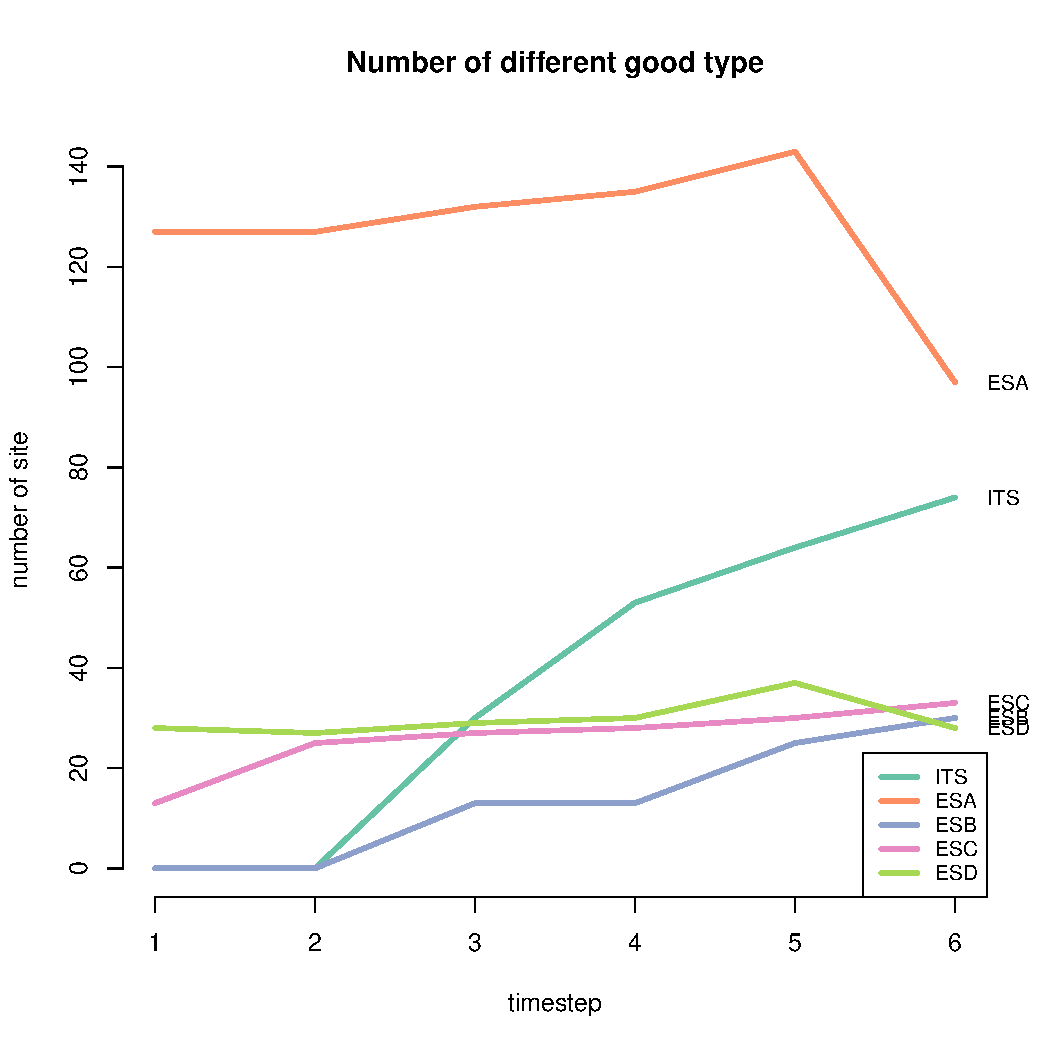
\includegraphics[width=.45\textwidth]{../images/plotNbSiteWGoodData.pdf}
     
 \end{figure}
 \begin{center}
     \tiny other info: Site with different number of goods
 \end{center}
\end{frame}



\begin{frame}{}
    \centering
    \Huge
    \bf
    What can explain those patterns?
\end{frame}

\begin{frame}{Structure of Economy}
    Brughmans \& Poblome (2016) Antiquity
    \begin{itemize}
	\item<1-> Nature of Economic interactions
	\begin{center}
		\uncover<2->{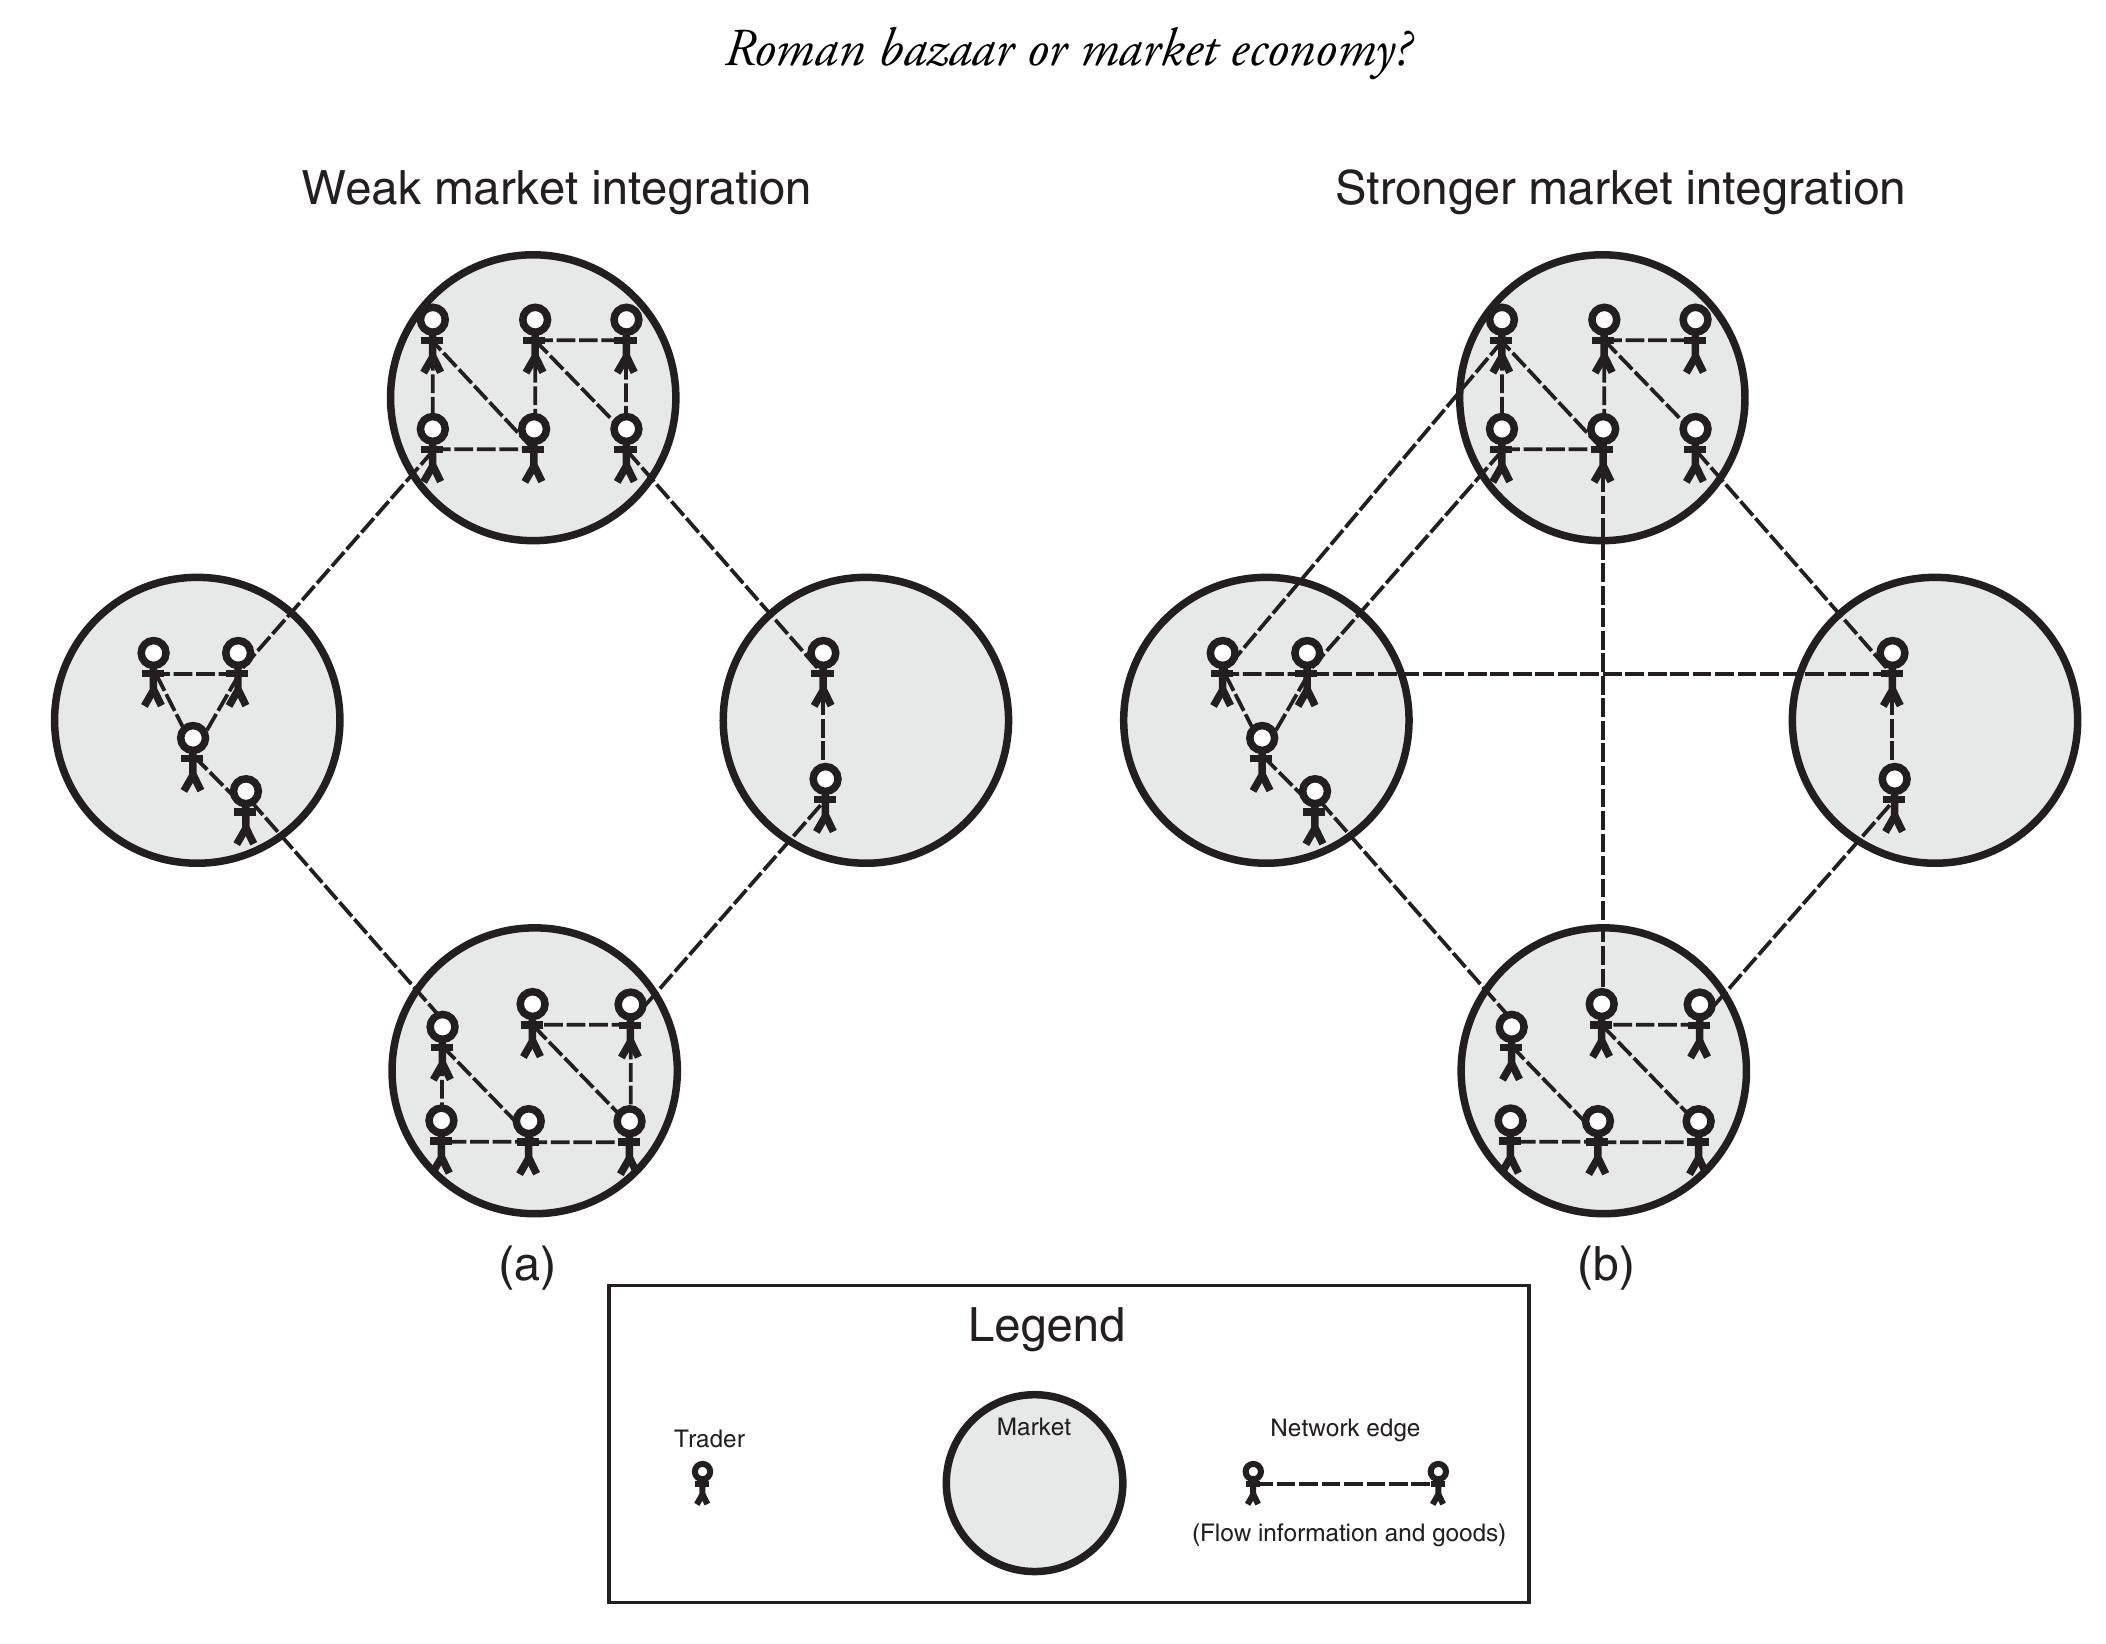
\includegraphics[width=.6\textwidth]{images/poblomeMarket}}
	\end{center}
    \end{itemize}
    \uncover<3->{$\rightarrow$ weak market integration \emph{cannot} reproduce the observed pattern}
\end{frame}

\begin{frame}{Another approach}
     Integrate social-cultural mechanisms to economic interactions:
    \uncover<2->{
	\begin{center}
	    \bf
	    The Cultural Evolution approach
	\end{center}
    }


    
\end{frame}



\begin{frame}{Cultural Evolution}
    \begin{itemize}
	\item<5->{ similar patterns}
	\item<6->{ apparition/disappearance of new trends,fluctuations\dots}
    \end{itemize}
	\begin{center}
		\uncover<4->{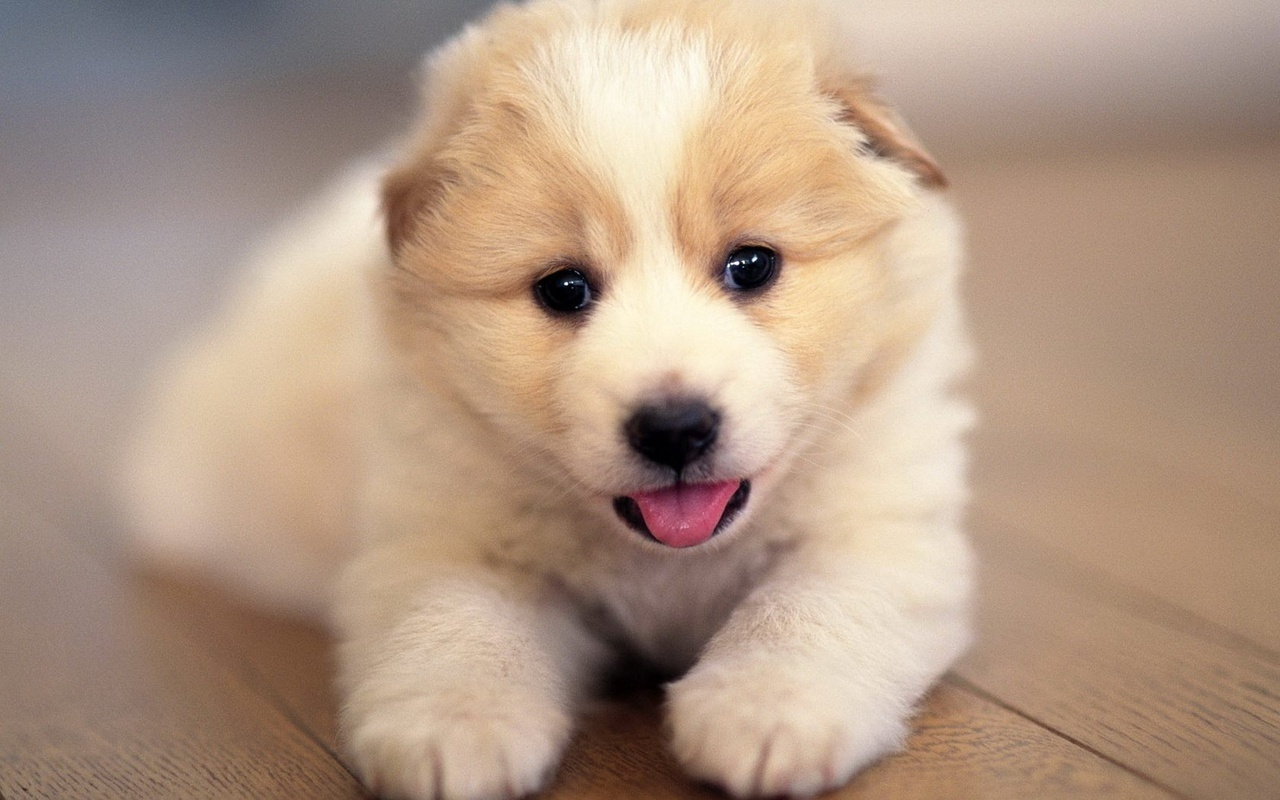
\includegraphics[width=3cm]{images/cutdog}}\\
		\vspace{.5cm}
		\uncover<2->{\includegraphics[width=2.5cm]{images/cutbaby}}
	    \hspace{1cm}
	    \uncover<3->{ \includegraphics[width=2cm]{images/pottery}}
	\end{center}
\end{frame}

\begin{frame}{What Generates Those Cultural changes?}
    $\rightarrow$ What mechanisms drive the evolution of such traits?\\
    \invisible<1->{$\rightarrow$ What mechanisms }generate such pattern?

    \vspace{1cm}

    \uncover<2->{Social-cultural mechanisms:\\}
	\begin{itemize}
	    \item<3->Individual learning: I learn by my own error - I suddenly have a new idea (\emph{ie} ``innovation''). 
		\item<4-> Social learning : I learn by exchanging with the other - by watching them. 
	\end{itemize}
\end{frame}

\begin{frame}{Neutral Model}
    Inspired by evolutionary biology:
    \begin{itemize}
	\item<2->Individual learning: random innovation
	\item<3-> Social learning : random/biased copy of something existing
    \end{itemize}

    
\end{frame}

\begin{frame}{Contemporary Examples}
	Distribution of names in the US (Bentley et al, 2004):\\
	\uncover<2->{\begin{figure}
		\begin{columns}
			\begin{column}{.8\textwidth}
				\centering
				\includegraphics[width=.6\textwidth]{images/powerlawrepartition.jpg}
			\end{column}
			\begin{column}{.3\textwidth}
				\tiny
				Square: male names\\
				Circle: female names\\
				Dotted and plain lines: model result with different copy probabilities.\\
			From Bentley et al,~2004.
			\end{column}
		\end{columns}
	    \end{figure}}
\end{frame}

\begin{frame}{Archaeological Examples}
	Non-functional attribute  of ceramics (Steele et al, 2010):\\
	\begin{figure}
		\begin{columns}
			\begin{column}{.7\textwidth}
				\centering
				\uncover<3->{	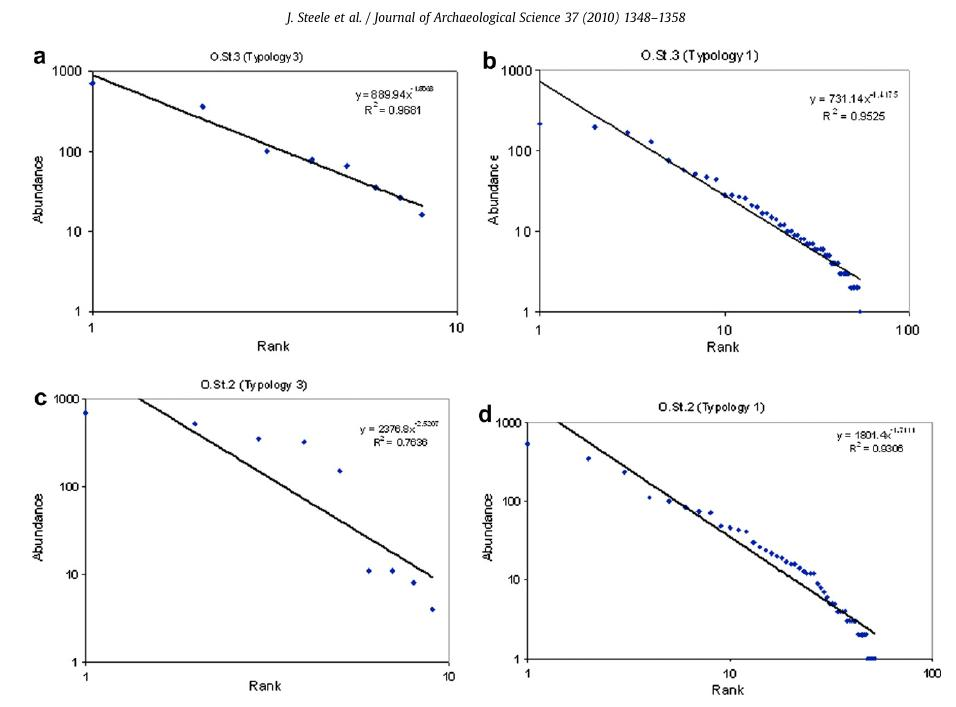
\includegraphics[width=1\textwidth]{images/steeletal2010Distrib.jpg}}
			\end{column}
			\begin{column}{.3\textwidth}
			    \uncover<2->{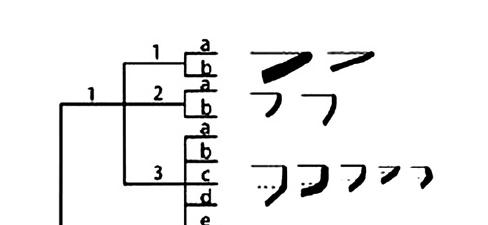
\includegraphics[width=1\textwidth]{images/steeletal2010rim}\\\vspace{.5cm}
				\tiny Distribution of variants for different bowl types given some slight diff. on the rim
			    }
			\end{column}
		\end{columns}
	    \end{figure}
\end{frame}


\begin{frame}{``Neutral'' model }
    Assumes :
    \begin{itemize}
	\item<+-> no functional difference
	\item<+-> Simple frequency-based bias (conformism, anti-conformism bias, no preference, prestige\dots)
	\item<+-> negligible economic cost 
	    \begin{itemize}
		\item<+-> production cost
		\item<+-> importation cost
		\item<+-> \dots

	    \end{itemize}
    \end{itemize}
    
\end{frame}

\section{Economic Traits}


\begin{frame}
	\begin{center}
	    \bf
	    \Huge
	    What if such mechanisms are explicitly linked to economics?
	\end{center}
\end{frame}

\begin{frame}{A social trait and economic value}
	\begin{center}
	    \only<1>{\includegraphics[width=.8\textwidth]{images/boubou1.png}}
	    \only<2>{\includegraphics[width=.8\textwidth]{images/boubou2.png}}
	    \only<3>{\includegraphics[width=.8\textwidth]{images/boubou3.png}}
	\end{center}
\end{frame}

\begin{frame}{Co-evolution of Economy and Culture}

%How Simple Cultural Dynamics influence Economy That in turn will influence cultural dynamics.
    \vspace{2cm}
    \begin{center}
	\begin{overlayarea}{\textwidth}{\textheight}
	    \only<1>{\includegraphics[width=\textwidth]{images/map1.png}}
	    \only<2>{\includegraphics[width=\textwidth]{images/map2.png}}
	    \only<3>{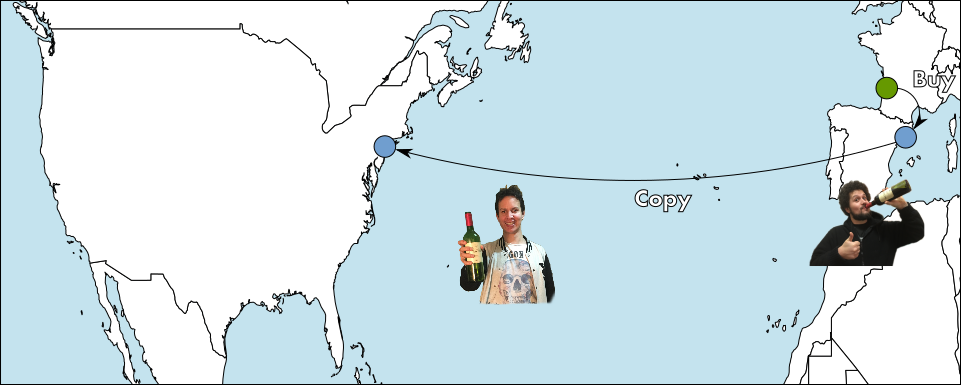
\includegraphics[width=\textwidth]{images/map3.png}}
	    \only<4>{\includegraphics[width=\textwidth]{images/map4.png}}
	    \only<5>{\includegraphics[width=\textwidth]{images/map5.png}}
	    \only<6>{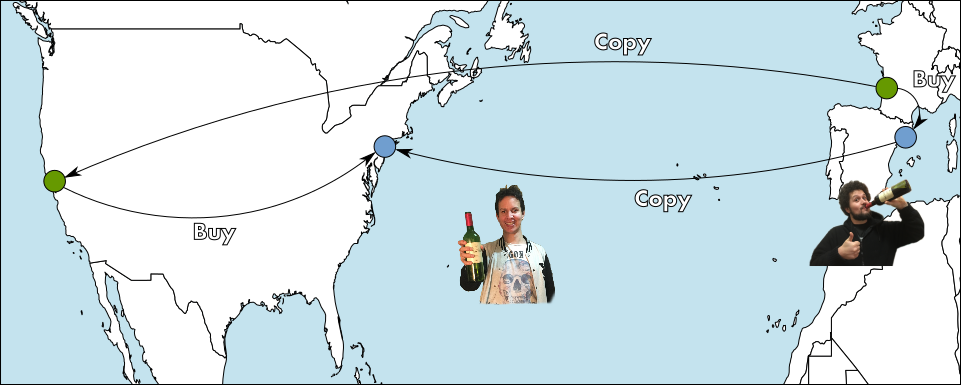
\includegraphics[width=\textwidth]{images/map6.png}}
	    \only<7>{\includegraphics[width=\textwidth]{images/map7.png}}
	    \only<8>{\includegraphics[width=\textwidth]{images/map8.png}}
	    \only<9>{\includegraphics[width=\textwidth]{images/map9.png}}
	\end{overlayarea}

    \end{center}
\end{frame}

\begin{frame}{Another Example}
	\begin{center}
	    \only<1>{\includegraphics[width=.8\textwidth]{images/boubou1.png}}
	    \only<2>{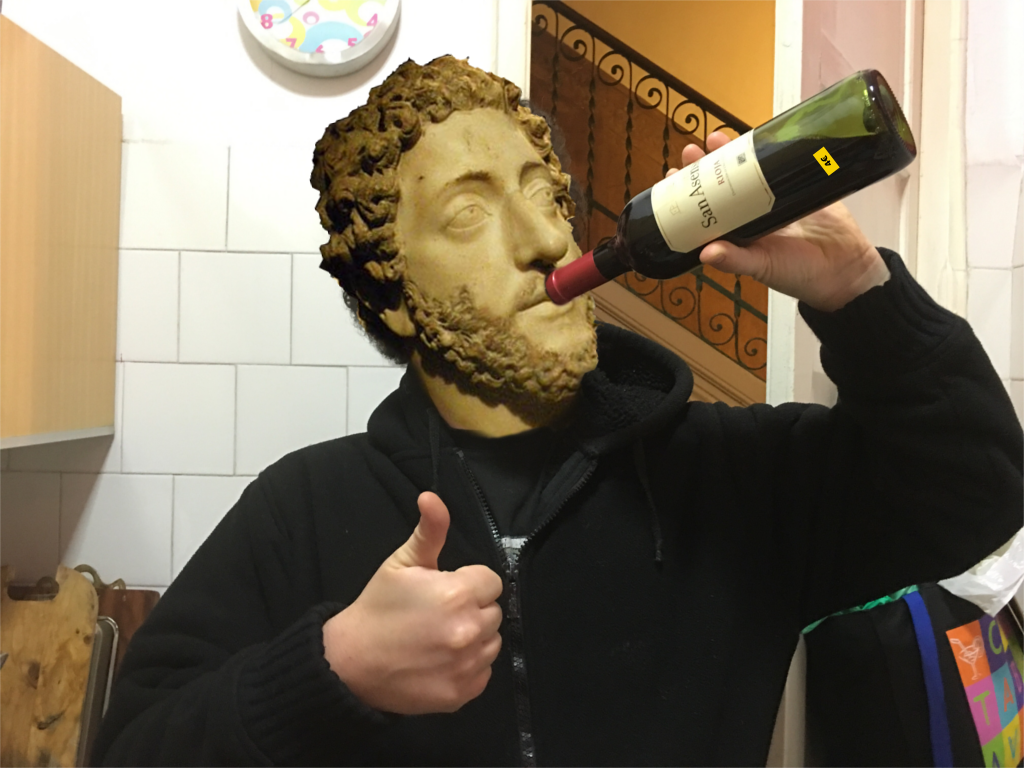
\includegraphics[width=.8\textwidth]{images/boubou4.png}}
	\end{center}
\end{frame}

\begin{frame}{Co-evolution of Economy and Culture}

%How Simple Cultural Dynamics influence Economy That in turn will influence cultural dynamics.
    \vspace{2cm}
    \begin{center}
	\begin{overlayarea}{\textwidth}{\textheight}
	    \only<1>{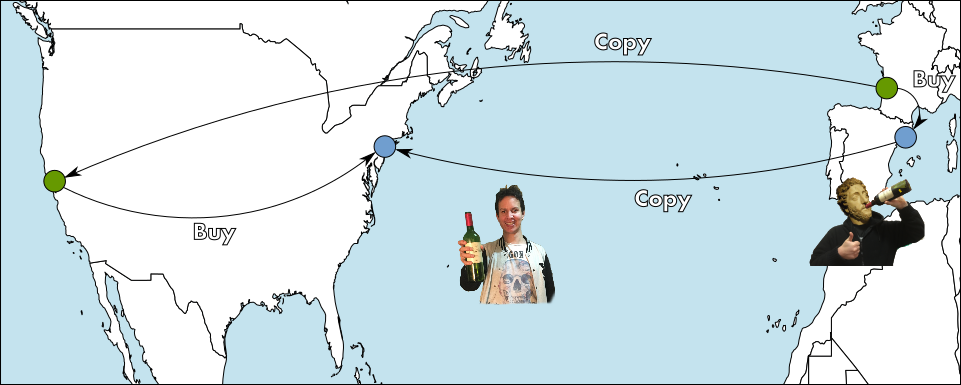
\includegraphics[width=\textwidth]{images/mapBis1}}
	    \only<2>{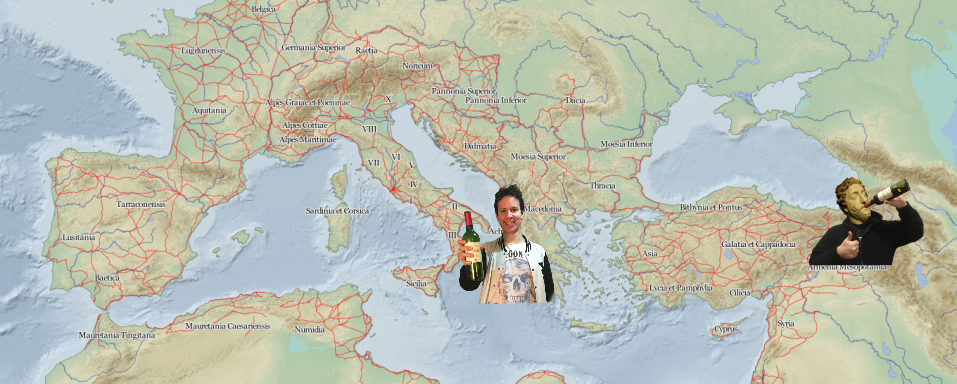
\includegraphics[width=\textwidth]{images/mapBis2}}
	    \only<3>{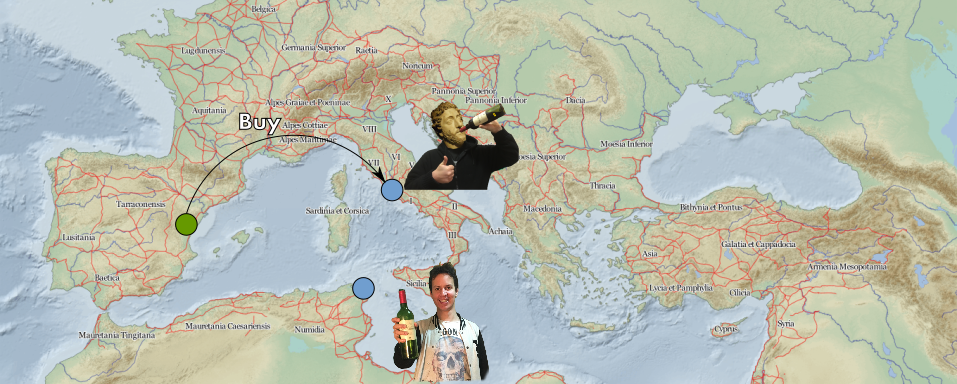
\includegraphics[width=\textwidth]{images/map3bBis}}
	    \only<4>{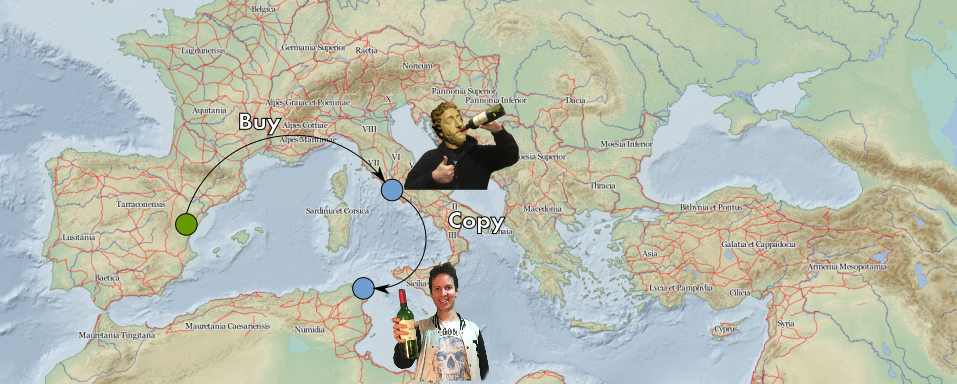
\includegraphics[width=\textwidth]{images/mapBis3}}
	    \only<5>{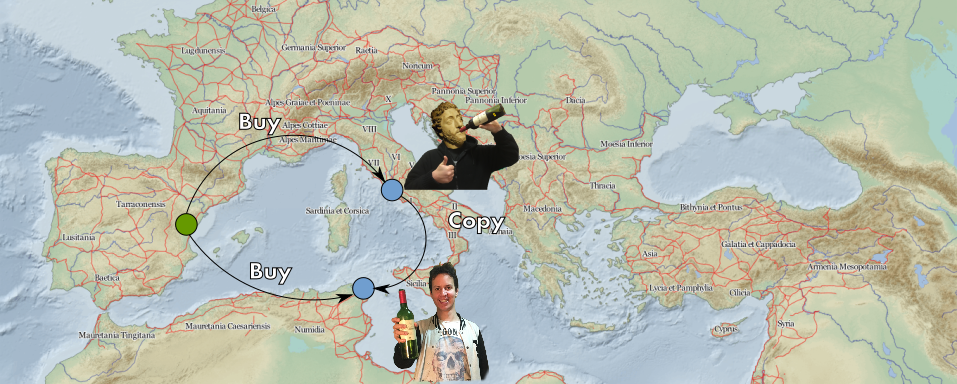
\includegraphics[width=\textwidth]{images/mapBis4}}
	    \only<6>{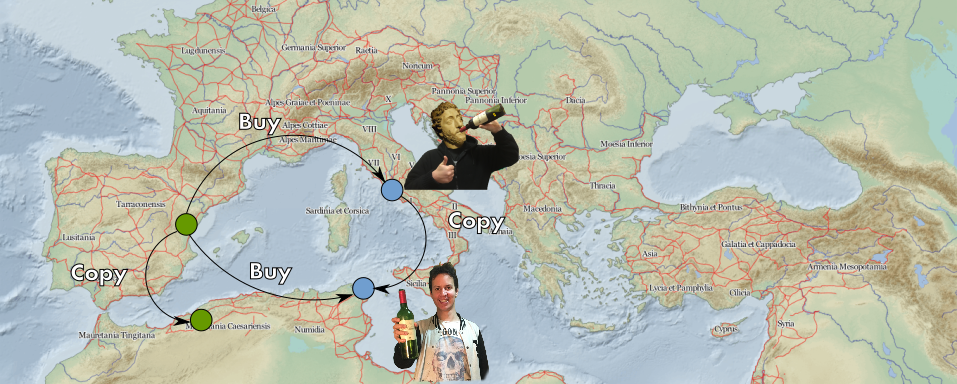
\includegraphics[width=\textwidth]{images/mapBis6}}
	    \only<7>{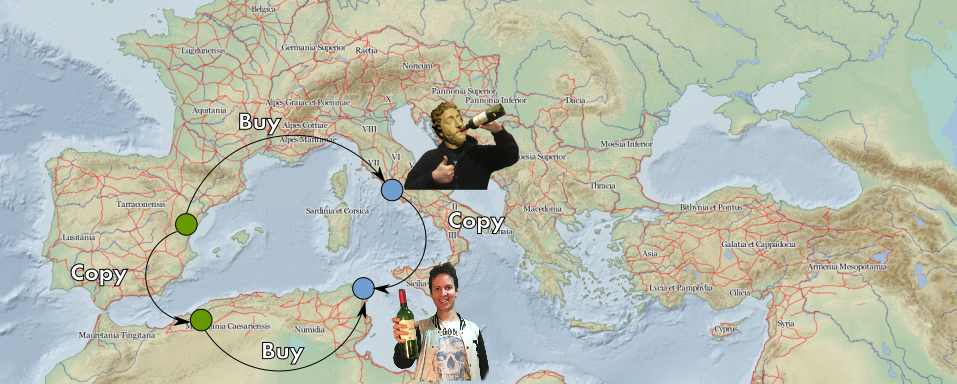
\includegraphics[width=\textwidth]{images/mapBis7}}
	    \only<8>{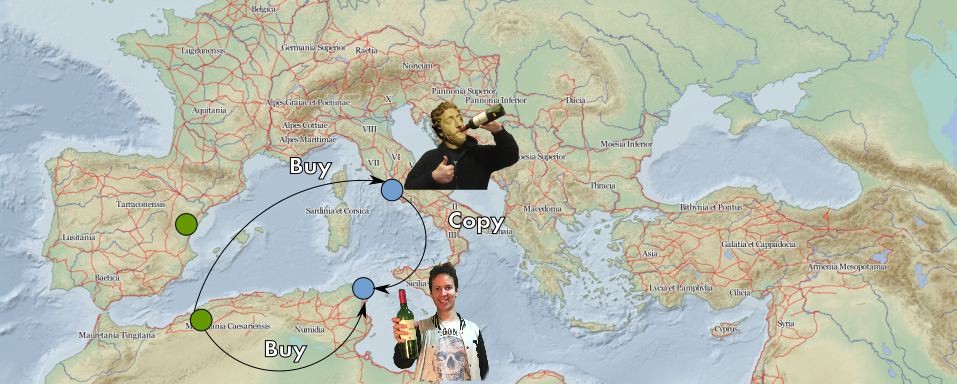
\includegraphics[width=\textwidth]{images/mapBis8}}
	    \only<9>{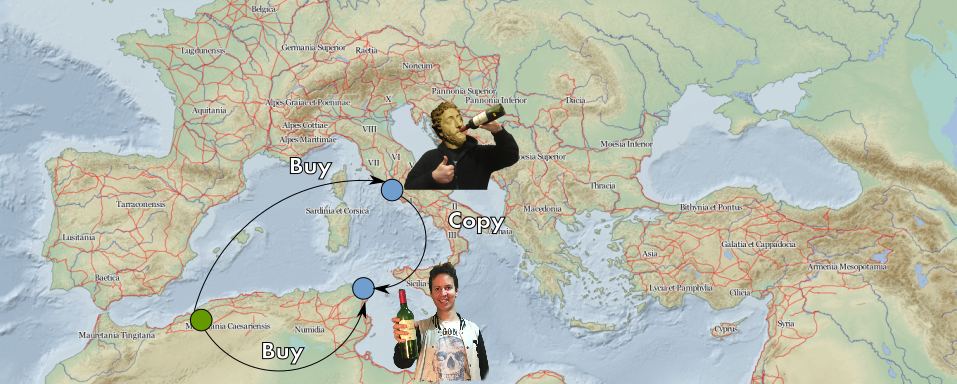
\includegraphics[width=\textwidth]{images/mapBis9}}
	\end{overlayarea}

    \end{center}
\end{frame}


\section{ABM Framework}


\begin{frame}{General Framework}
    
    \begin{center} 
	\includegraphics[width=.8\textwidth]{images/cooev.png}	
    \end{center}
\end{frame}

\begin{frame}{Computer Model}
    \vfill
    \begin{center}
	\includegraphics<+->[width=.5\textwidth]{images/cooev.png}	
    \end{center}
    \uncover<+->{Agent Based Model}
    \vfill
	\begin{itemize}
	\item<+-> Different cultural transmission mechanisms
    \vfill
	\item<+-> Different trade assumptions
    \vfill
	\item<+-> Historical and Archaeological evidences 
    \vfill
	\item<+-> Network Constraints
    \vfill
	\item<+-> \dots
    \vfill
	\end{itemize}
\end{frame}
	
\begin{frame}{Agent Based Model}
    
\uncover<+->{Already implemented and studied at theoretial (Carrignon et al. 2016, Gintis 2006, Chen et al. 2017}
    \begin{itemize}
	\item<+-> Simple decentralized economy
	\item<+-> Agents produce and exchange goods
	\item<+-> Agents are ranked givent ``their economic success''
	\item<+-> Agents can socially learn form each other and ``innovate''
	\item<+-> Reach Walrasian ``general equilibrium'' when agents copy the best 
    \end{itemize}
\end{frame}


\begin{frame}{Economic Dynamics}
	\begin{figure}
	    \caption{Example for 3 goods and 500 agents}
	    \begin{columns}
		\column{.5\textwidth}
		\includegraphics[height=\textwidth]{images/ClearingPriceDistanceEvolutionForTrade-G3N500.pdf}\\
	    \end{columns}
		@~Equilibrium: personal values  $\rightarrow$ optimal (shared) values.
	\end{figure}
	
\end{frame}



\begin{frame}{ICRATES}
    \footnotesize
    \vspace{.5cm}
Change in distribution of Tableware in the  Roman East, -25BC 150AD:
    \begin{itemize}
	\item 5 types of wares 
	\item Distribution among 222 sites
	\item 5121 ware dataset
 \end{itemize}

 \begin{figure}
     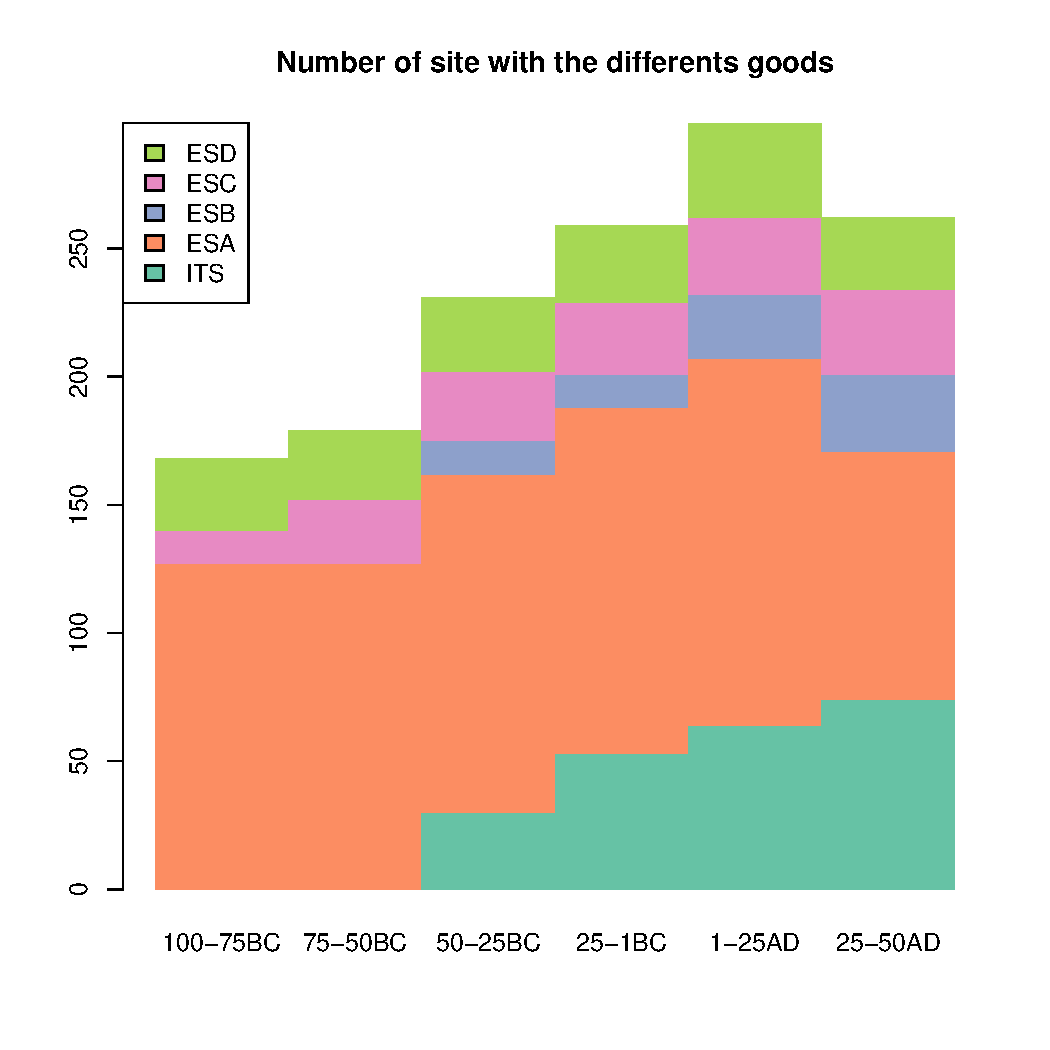
\includegraphics[width=.45\textwidth]{../images/hmNbSiteWGoodData.pdf}
     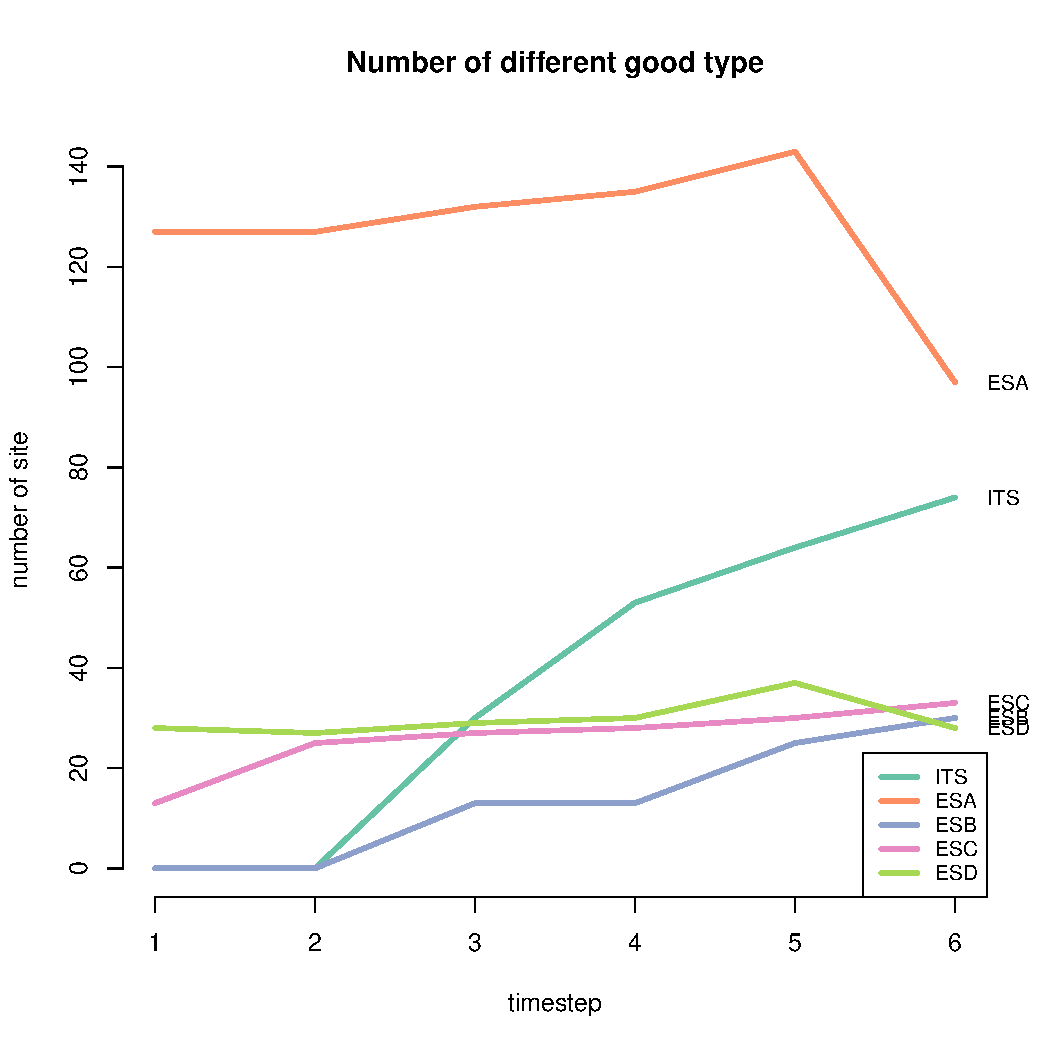
\includegraphics[width=.45\textwidth]{../images/plotNbSiteWGoodData.pdf}
     
 \end{figure}
\end{frame}

\begin{frame}{Specification of the model}
    \uncover<+->{ { \bf A case study and a model}\\}
    \vspace{1cm}
    \uncover<+->{\textcolor{UPF}{\textbf{1. }\Huge}Integrate historical knowledge: \\
$\rightarrow$ Calibrate the model to produce more ``realistic'' simulations}
	    \begin{itemize}
		\item<+-> 5 different types of good 
		\item<+-> Goods appear one after this other
		\item<+-> Agents are markets of urban settlements
		\item<+-> Number of agents based on historical estimations
	    \end{itemize}
    
\end{frame}

\begin{frame}{Individual vs Social learning}

    %We can now precise: \textbf{individual} vs \textbf{social}  learning\\
    \textcolor{UPF}{\textbf{2. }\Huge}Agents as markets of urban settlements:
    \begin{itemize}
	\item<2-> \textbf{individual} learning (innovation): \\
	    \uncover<3->{ \hspace{.5cm} $\rightarrow$ the capacity of a market to generate new solutions by itself (internal changes, interactions within a market: \emph{ie} \textbf{creativity}) } 
	\item<4-> \textbf{social} learning (cultural transmission): \\
	    \uncover<5->{ \hspace{.5cm} $\rightarrow$ the tendency of a market to copy another (better) one (interactions, communication between markets: \emph{ie} \textbf{openness}) }
    \end{itemize}
\end{frame}

\begin{frame}{Experimental framework}

\textcolor{UPF}{\textbf{3. }\Huge}\uncover<+->{Experimental setup, test the importance of those factors:}
    \begin{itemize}
	\item<+-> 	    \textbf{Individual learning}/creativity: ``a settlement decides to change the value of a ware''\\
	    \uncover<+->{$\mu \rightarrow$ increase the probability of creating a new solution\\}

	    \uncover<+->{\hspace{.2cm} $\mu \in \{0.001,0.01,0.1,1\}$}
	\item<+-> 	    \textbf{Social learning}/openness:``a market decide to copy another, more successful market''\\
	    \uncover<+->{$\lambda\rightarrow$ increase the probability to copy a more successful settlement\\}

	    \uncover<+->{\hspace{.2cm} $\lambda \in \{0.0001,0.001,0.01,0.1,1,10\}$}
	\item<+->  $ 6 \times 4 = 24$ setup, 50s simulation each
    \end{itemize}
\end{frame}


\begin{frame}{Result}
    1200 Simulations for different pairs of parameters.
    \begin{table}
	\centering

	\begin{tabular}{rr|cccc}
	    & &\multicolumn{4}{c}{ $\mu$ } \\
	    & & $0.001$ & $0.01$ & $0.1$ & $1$ \\ \hline
	    \multirow{6}{*}{$\lambda$} 
	    & 0.0001	& $\times50$ & $\times50$ & $\times50$ & $\times50$ \\
	    & 0.001	& $\times50$ & $\times50$ & $\times50$ & $\times50$ \\
	    & 0.01	& $\times50$ & $\times50$ & $\times50$ & $\times50$ \\
	    & 0.1	& $\times50$ & $\times50$ & $\times50$ & $\times50$ \\
	    & 1		& $\times50$ & $\times50$ & $\times50$ & $\times50$ \\
	    & 10	& $\times50$ & $\times50$ & $\times50$ & $\times50$ 
	\end{tabular}
    \end{table}

\end{frame}

\begin{frame}{Result}

    \tikzset{
	every picture/.style={remember picture,baseline},
	every node/.style={
	    inner sep=0pt,
	    anchor=base,
	    minimum width=1.8cm,
	    align=center,
	    text depth=.25ex,
	outer sep=1.5pt},
	every path/.style={
	    thick, 
	    rounded corners
	}
    }  
    1200 Simulations for different pairs of parameters.

    \begin{table}
	\center
	\begin{tabular}{rrcccc}
	    & &\multicolumn{4}{c}{ creativity } \\
	    & &\multicolumn{1}{|c}{\tiny $--$ } & \multicolumn{2}{c}{ \tiny \dots }& \tiny $++$ \\\cline{2-6}
	    \multirow{6}{*}{\rotatebox[origin=c]{90}{openness}} 
	    & \multirow{2}{*}{\tiny $--$}
	    		& \multicolumn{1}{|c}{$\times50$ } & $\times50$ & $\times50$ & $\times50$ \\
			& 		& \multicolumn{1}{|c}{$\times50$ } & $\times50$ & $\times50$ & \tabnode{$\times50$} \\
	    & \multirow{2}{*}{\tiny \dots}
	    		& \multicolumn{1}{|c}{$\times50$ } & $\times50$ & $\times50$ & $\times50$ \\
	    & 		& \multicolumn{1}{|c}{$\times50$ } & $\times50$ & $\times50$ & $\times50$ \\
	    & \multirow{2}{*}{\tiny $++$}
	    		& \multicolumn{1}{|c}{$\times50$ } & $\times50$ & $\times50$ & $\times50$ \\
			& 	& \multicolumn{1}{|c}{ \tabnode{$\times50$} } & $\times50$ & $\times50$ & $\times50$ 
	\end{tabular}
    \end{table}

    \begin{tikzpicture}[remember picture,overlay]
	\draw<2-> (1) ellipse (.42cm and .33cm) [red];
	\node<3->[right=.5cm,minimum width=0pt,red] at (1) (A) {ExpB};
	\draw<4-> (2) ellipse (.42cm and .33cm) [red];
	\node<5->[below=.5cm,minimum width=0pt,red] at (2) (B) {ExpG};
	\end{tikzpicture}
\end{frame}

\begin{frame}{Exemple}
    \small
    \centering
    \begin{table}
	\begin{tabular}{ccc}
	    Data 	&  ExpG {\tiny ($\lambda=0.001,\mu=1$)} &  ExpB {\tiny ($\lambda=10,\mu=0.001$)}   \\
	    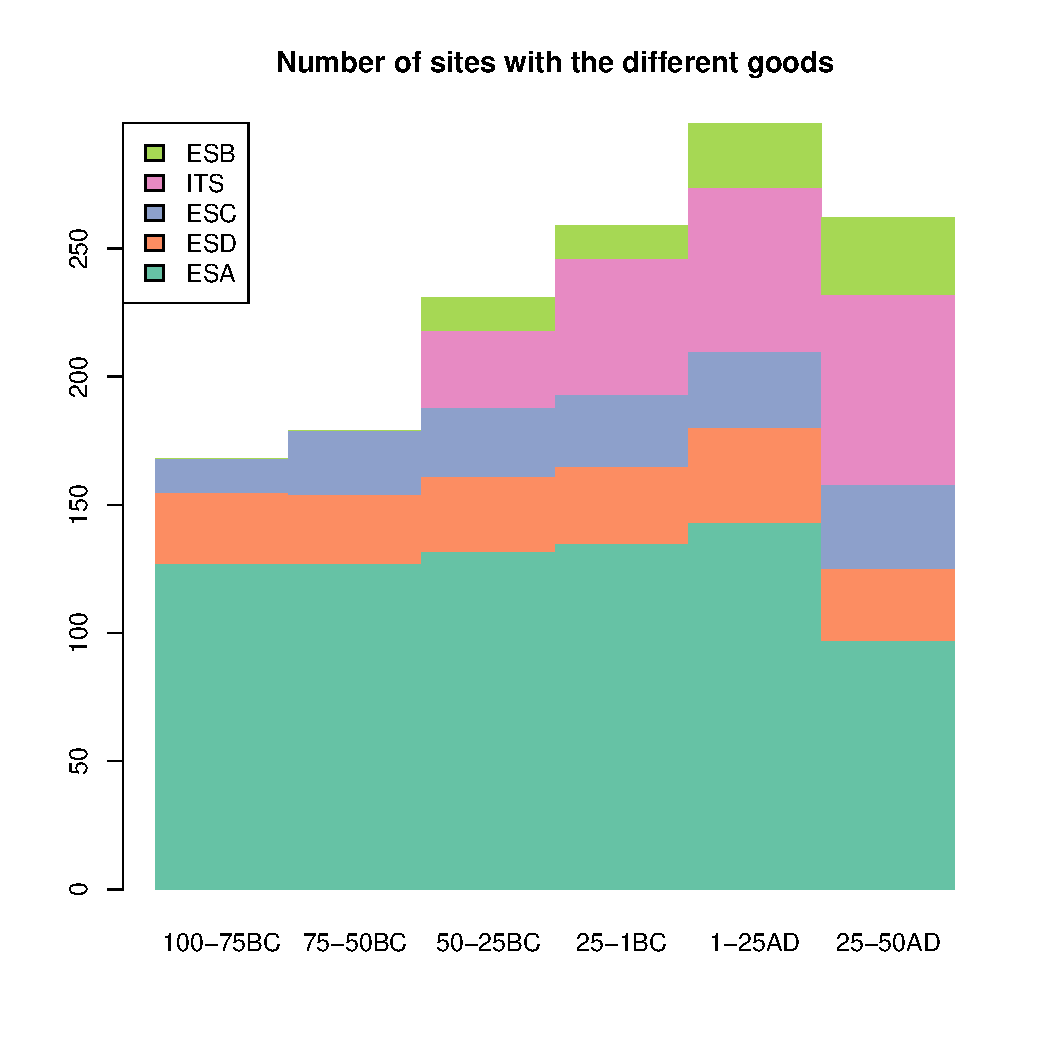
\includegraphics[width=.3\textwidth]{images/hmData.pdf}	&
	    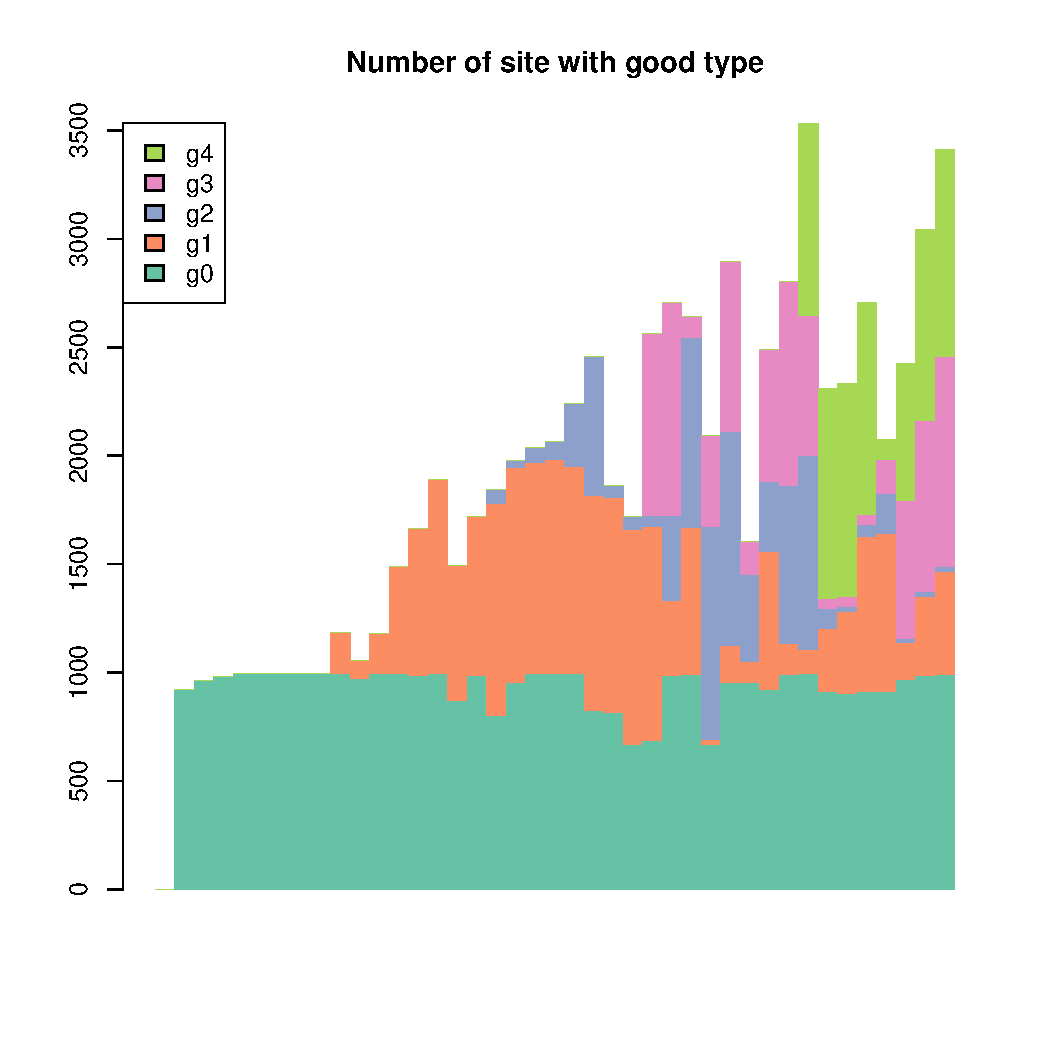
\includegraphics[width=.3\textwidth]{images/hmGoodSimu.pdf}	&
	    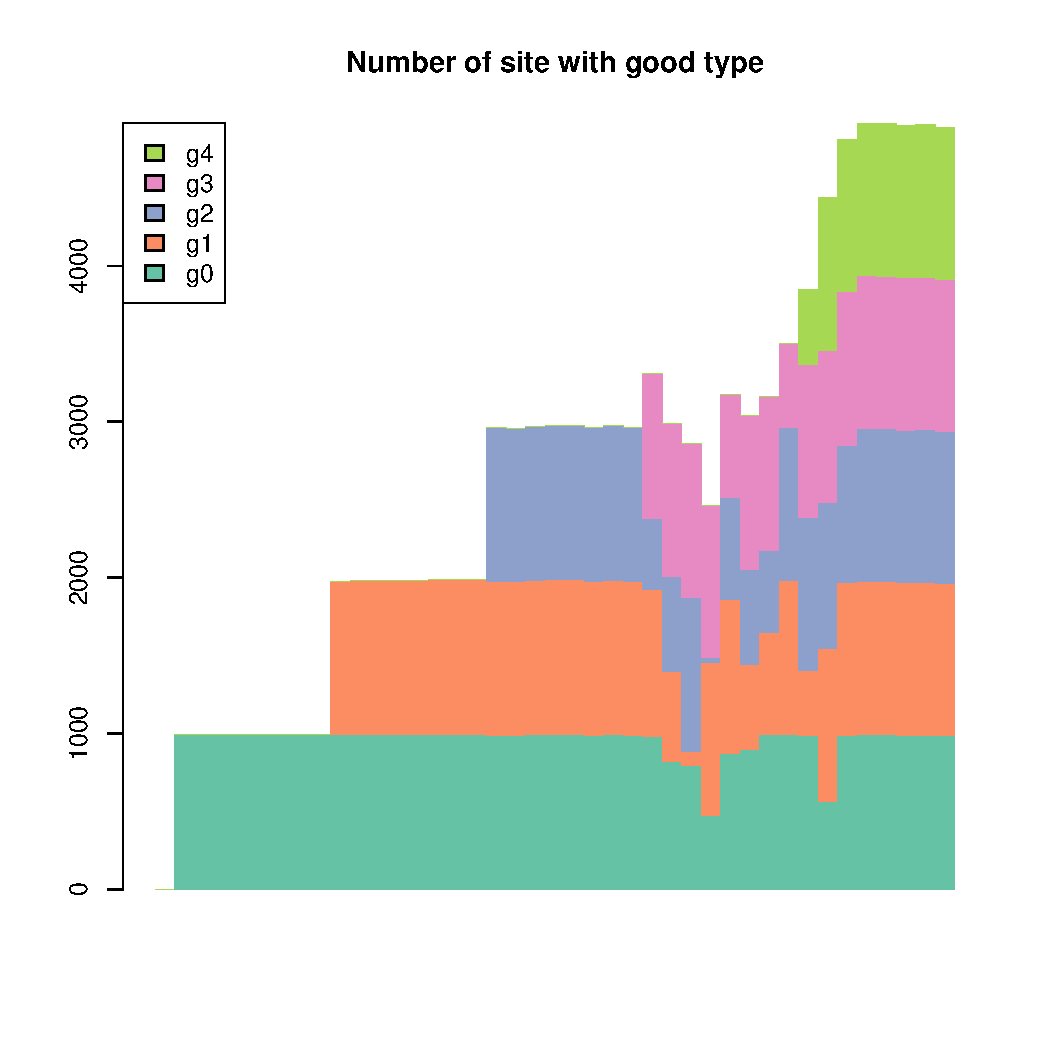
\includegraphics[width=.3\textwidth]{images/hmBadSimu.pdf}	\\
	    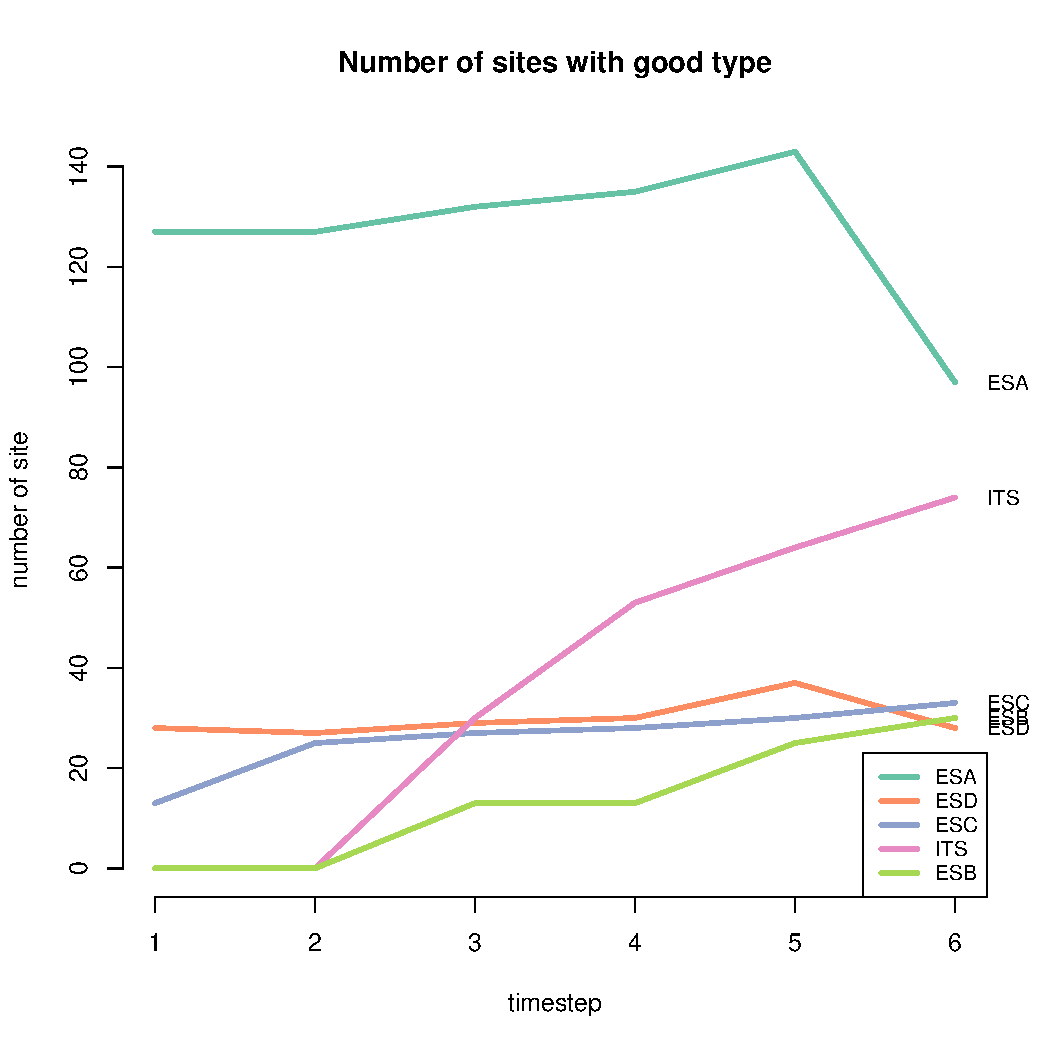
\includegraphics[width=.3\textwidth]{images/plotData.pdf}	&
	    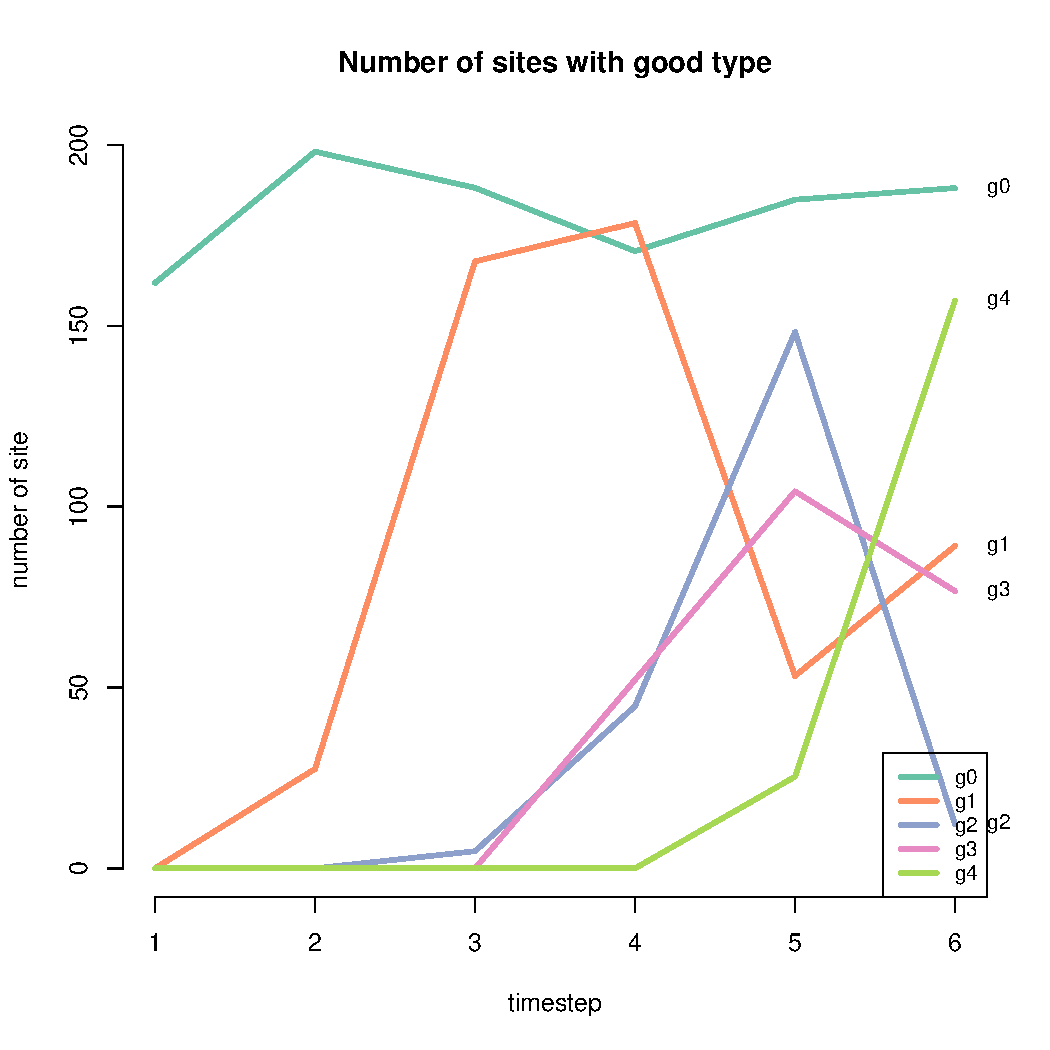
\includegraphics[width=.3\textwidth]{images/plotGoodSimu.pdf}	&
	    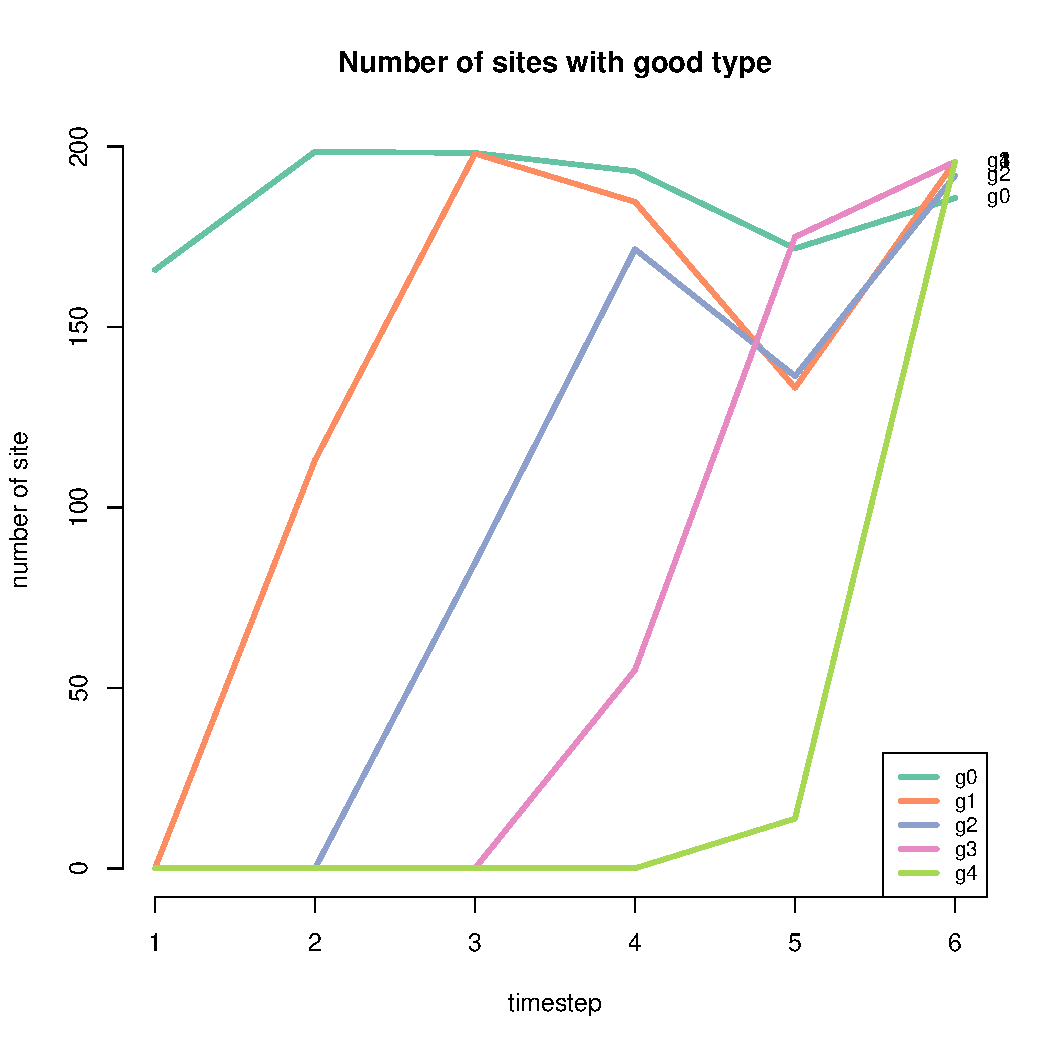
\includegraphics[width=.3\textwidth]{images/plotBadSimu.pdf}	\\

	\end{tabular}
    \end{table}
\end{frame}


\begin{frame}{Compare Simulations with Data}
    \centering
	    Data\\
	    \includegraphics<1>[width=.3\textwidth]{images/plotData.pdf}  
	    \includegraphics<2-4>[width=.3\textwidth]{images/plotData1.pdf}
	    \includegraphics<5-7>[width=.3\textwidth]{images/plotData2.pdf}
	    \includegraphics<8-10>[width=.3\textwidth]{images/plotData3.pdf}
	    \includegraphics<11-13>[width=.3\textwidth]{images/plotData4.pdf}
	    \includegraphics<14-16>[width=.3\textwidth]{images/plotData5.pdf}
	    \includegraphics<17->[width=.3\textwidth]{images/plotData.pdf}  

	\begin{tabular}{cc}
	    ExpG & ExpB\\
	    \includegraphics<1>[width=.3\textwidth]{images/plotGoodSimu.pdf}  

	    \includegraphics<2>[width=.3\textwidth]{images/plotGoodSimu1A.pdf}
	    \includegraphics<3>[width=.3\textwidth]{images/plotGoodSimu1B.pdf}
	    \includegraphics<4>[width=.3\textwidth]{images/plotGoodSimu1C.pdf}

	    \includegraphics<5>[width=.3\textwidth]{images/plotGoodSimu2A.pdf}
	    \includegraphics<6>[width=.3\textwidth]{images/plotGoodSimu2B.pdf}
	    \includegraphics<7>[width=.3\textwidth]{images/plotGoodSimu2C.pdf}

	    \includegraphics<8>[width=.3\textwidth]{images/plotGoodSimu3A.pdf}
	    \includegraphics<9>[width=.3\textwidth]{images/plotGoodSimu3B.pdf}
	    \includegraphics<10>[width=.3\textwidth]{images/plotGoodSimu3C.pdf}

	    \includegraphics<11>[width=.3\textwidth]{images/plotGoodSimu4A.pdf}
	    \includegraphics<12>[width=.3\textwidth]{images/plotGoodSimu4B.pdf}
	    \includegraphics<13>[width=.3\textwidth]{images/plotGoodSimu4C.pdf}

	    \includegraphics<14>[width=.3\textwidth]{images/plotGoodSimu5A.pdf}
	    \includegraphics<15>[width=.3\textwidth]{images/plotGoodSimu5B.pdf}
	    \includegraphics<16>[width=.3\textwidth]{images/plotGoodSimu5C.pdf}

	    \includegraphics<17>[width=.3\textwidth]{images/plotGoodSimu.pdf}  
	    \includegraphics<18>[width=.3\textwidth]{images/plotGoodSimuEnd.pdf}  

	    &

	    \includegraphics<1>[width=.3\textwidth]{images/plotBadSimu.pdf}  

	    \includegraphics<2>[width=.3\textwidth]{images/plotBadSimu1A.pdf}
	    \includegraphics<3>[width=.3\textwidth]{images/plotBadSimu1B.pdf}
	    \includegraphics<4>[width=.3\textwidth]{images/plotBadSimu1C.pdf}

	    \includegraphics<5>[width=.3\textwidth]{images/plotBadSimu2A.pdf}
	    \includegraphics<6>[width=.3\textwidth]{images/plotBadSimu2B.pdf}
	    \includegraphics<7>[width=.3\textwidth]{images/plotBadSimu2C.pdf}

	    \includegraphics<8>[width=.3\textwidth]{images/plotBadSimu3A.pdf}
	    \includegraphics<9>[width=.3\textwidth]{images/plotBadSimu3B.pdf}
	    \includegraphics<10>[width=.3\textwidth]{images/plotBadSimu3C.pdf}

	    \includegraphics<11>[width=.3\textwidth]{images/plotBadSimu4A.pdf}
	    \includegraphics<12>[width=.3\textwidth]{images/plotBadSimu4B.pdf}
	    \includegraphics<13>[width=.3\textwidth]{images/plotBadSimu4C.pdf}

	    \includegraphics<14>[width=.3\textwidth]{images/plotBadSimu5A.pdf}
	    \includegraphics<15>[width=.3\textwidth]{images/plotBadSimu5B.pdf}
	    \includegraphics<16>[width=.3\textwidth]{images/plotBadSimu5C.pdf}

	    \includegraphics<17>[width=.3\textwidth]{images/plotBadSimu.pdf}  
	    \includegraphics<18>[width=.3\textwidth]{images/plotBadSimuEnd.pdf}  
	    \\

	    \tiny
	    $\uncover<4->{\Delta_{ExpG} = A} \uncover<7->{ + B}\uncover<10->{ + C}\uncover<13->{ + D}\uncover<16->{ + E} \uncover<18->{ \approx 31} $ & 
	    \tiny 
	    $\uncover<4->{\Delta_{ExpB} = A'} \uncover<7->{ + B'}\uncover<10->{ + C'}\uncover<13->{ + D'}\uncover<16->{ + E'} \uncover<18->{ \approx 42} $ 





	\end{tabular}
	

    \end{frame}

\begin{frame}{Distribution of simulations scores}
    \begin{center}
	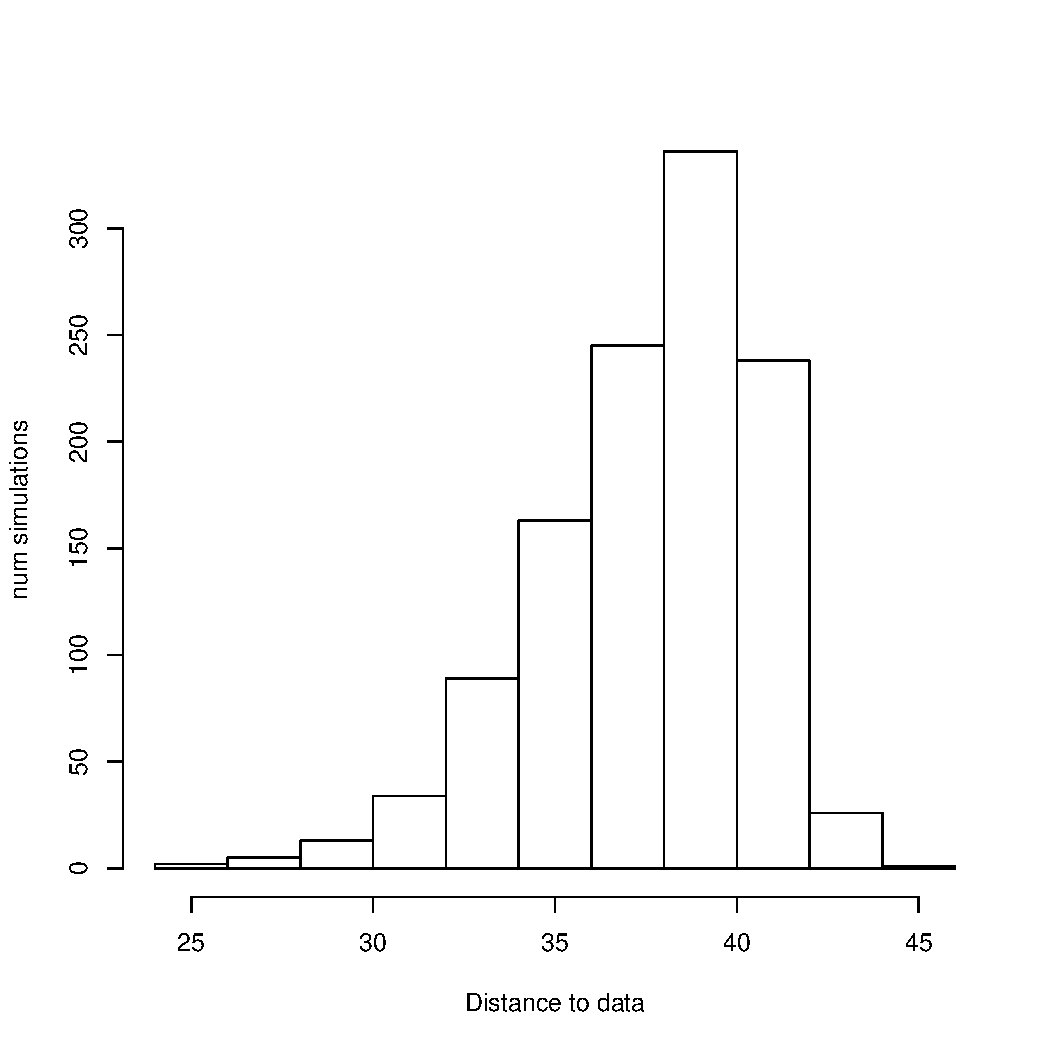
\includegraphics[width=.65\textwidth]{images/histScore.pdf}\\
    \end{center}
\end{frame}

\begin{frame}{Distribution of simulations scores}
    \begin{center}
	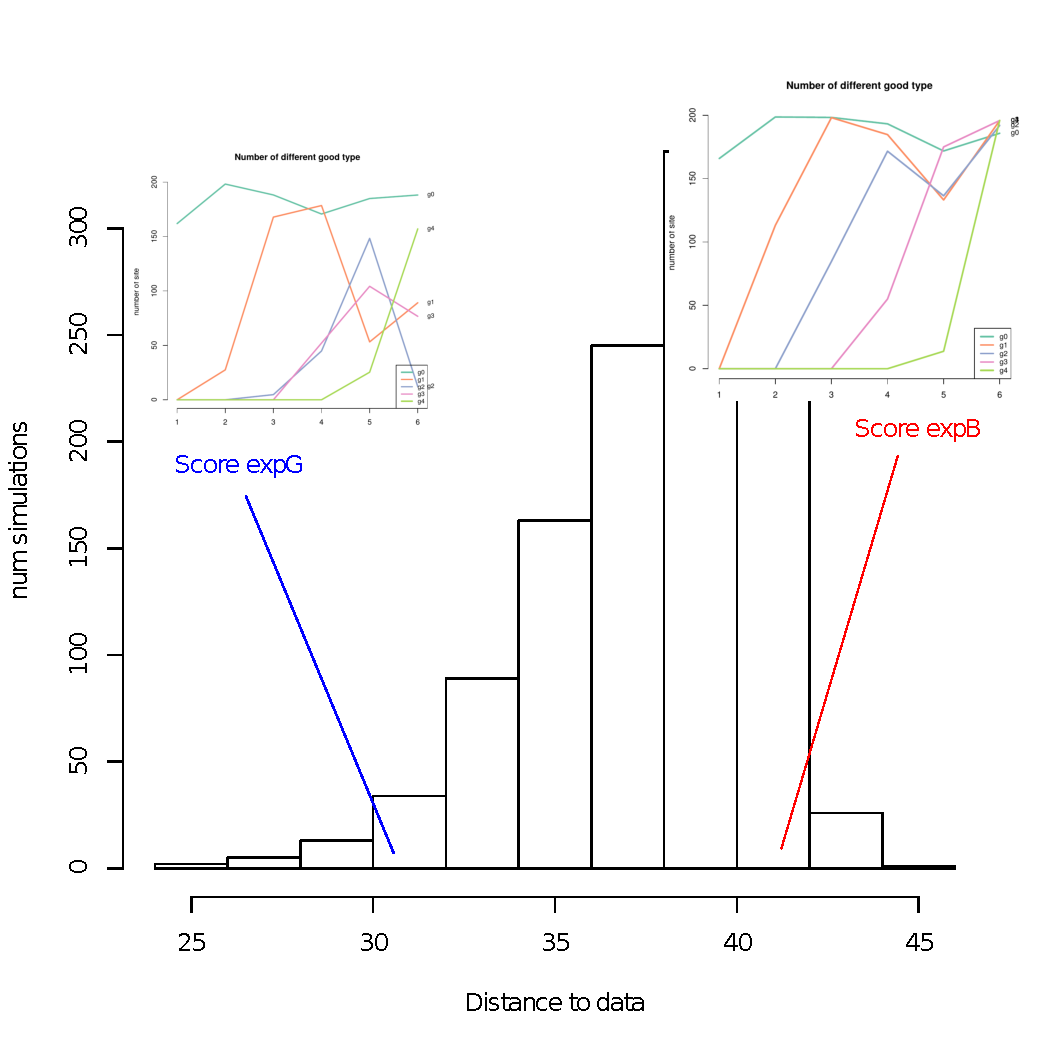
\includegraphics[width=.65\textwidth]{images/histScoreGB.pdf}\\
    \end{center}
\end{frame}

\begin{frame}{Compare pairs of parameters}

    \begin{center}
	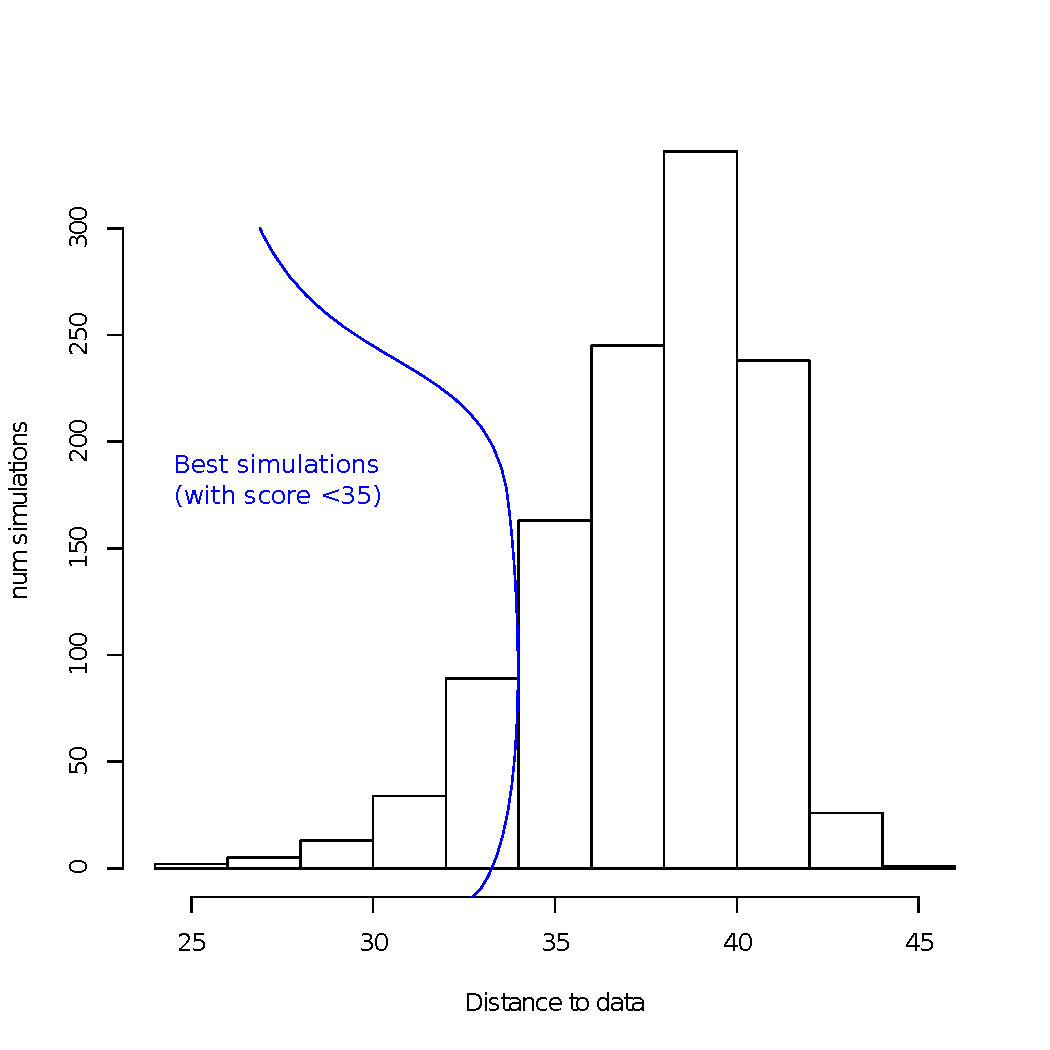
\includegraphics[width=.65\textwidth]{images/histScoreBest.pdf}\\
    \end{center}
    We select only the simulations ``more similar'' to the data.
\end{frame}

\begin{frame}{Compare pairs of parameters}
    For each pairs of parameters, we count how many simulations fall within this ``more similar'' threshold.
    \begin{figure}
	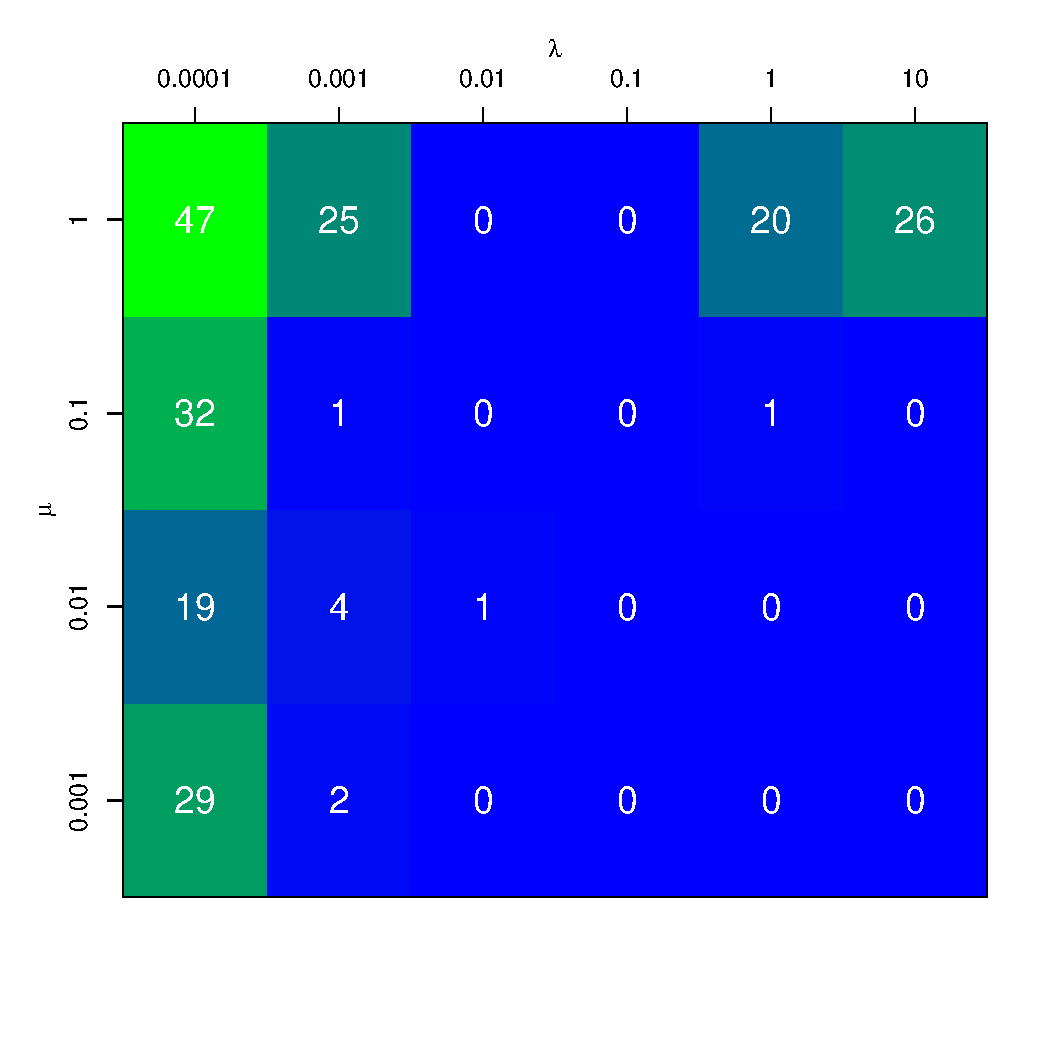
\includegraphics[width=.4\textwidth]{images/heatmapSimu}\\
	\centering
    \end{figure}

    \uncover<2->{Interpretation?
    \begin{itemize}
	\item <3-> Model not satisfying yet.
	\item <4-> \textcolor{UPF}{Very limited}
	\item <5-> But\dots
    \end{itemize}
}
\end{frame}

\begin{frame}{Interpretation}
    \begin{figure}
	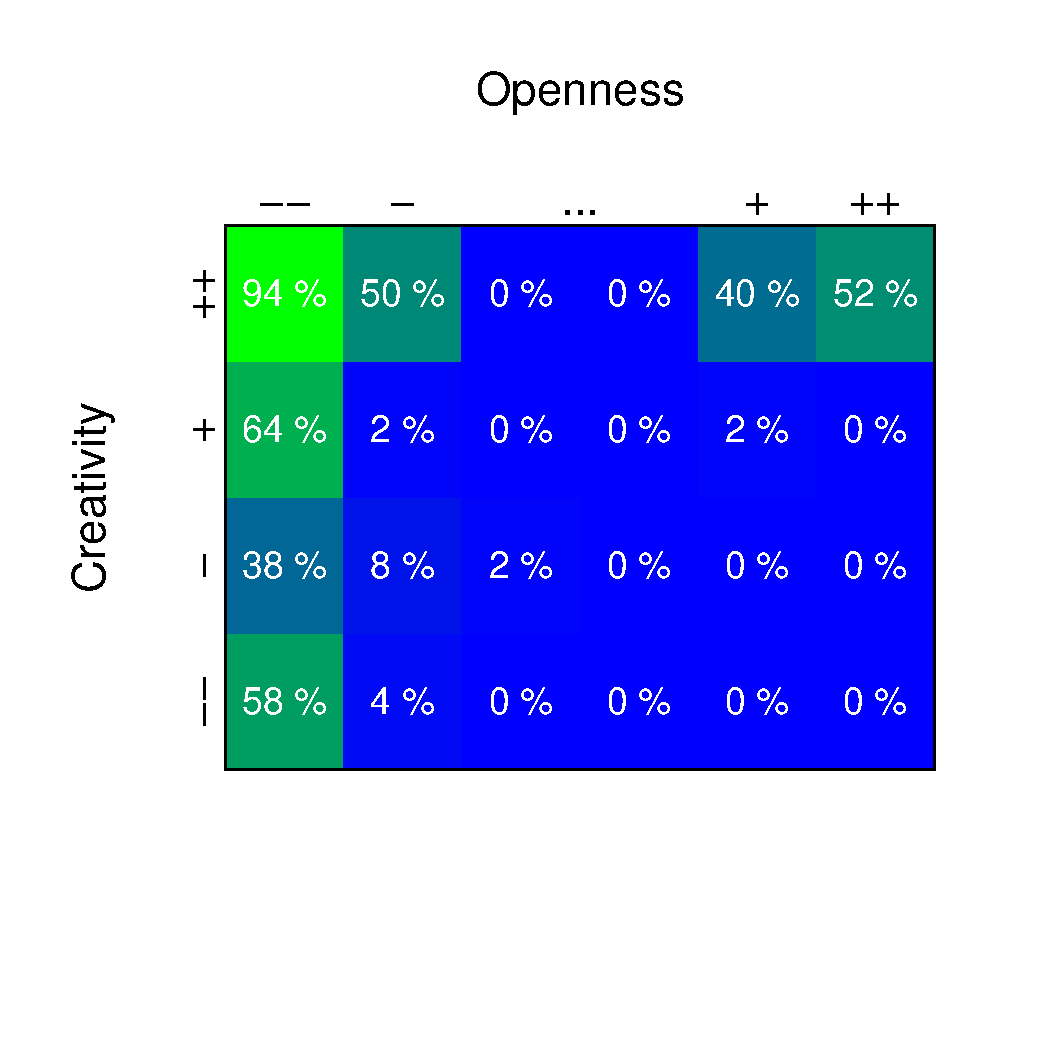
\includegraphics[width=.65\textwidth]{images/heatmapSimuProba.pdf}\\
	\centering
    \end{figure}

\end{frame}


%%%TODO
\begin{frame}{Limitations}
    {\tiny(beside the fact that the model isn't the good one yet)\\}
    \vspace{1cm}
    Heavily rely on expert knowledge:
    \begin{itemize}
	\item Every assumption counts :
	    \begin{itemize}
		\item The way we use the data
		\item How we defined when ``a experiment \emph{reproduce} the data''
	    \end{itemize}
	\item Interpretation is relative: compare hypothesis
    \end{itemize}

\end{frame}



\begin{frame}
	\begin{center}
		Thank you for you attention\\
%		What was the nature of Roman economy?\\
		\vspace{.5cm}
		\includegraphics[width=2cm]{images/LOGO-ERC.jpg} \hfil	\includegraphics[width=3cm]{../../logos/epnetLogo.png}\\
		\includegraphics[width=3cm]{images/leverhulme}\\
		\vspace{.5cm}
		\scriptsize
			http://www.roman-ep.net/\\
			@simoncarrignon
	\end{center}


\end{frame}

\end{document}


